\documentclass[conference]{IEEEtran}

% === Encodage, fontes, langue ===
\usepackage[utf8]{inputenc}
\usepackage[T1]{fontenc}
\usepackage[french]{babel}
\usepackage{csquotes}

% === Traductions des légendes en français (après IEEEtran) ===
\addto\captionsfrench{%
  \renewcommand{\tablename}{Tableau}%
  \renewcommand{\figurename}{Figure}%
  \renewcommand{\lstlistingname}{Code source}%
  \renewcommand{\refname}{Bibliographie}%
}

% === Maths & symboles ===
\usepackage{amsmath,amssymb,array}
\renewcommand{\arraystretch}{1.2}

% === Algorithmes ===
\usepackage{algorithm}
\usepackage{algpseudocode}
\floatname{algorithm}{Algorithme}
\renewcommand{\algorithmicrequire}{\textbf{Entrées :}}
\renewcommand{\algorithmicensure}{\textbf{Sorties :}}
\renewcommand{\algorithmicfor}{\textbf{Pour}}
\renewcommand{\algorithmicforall}{\textbf{Pour tout}}
\renewcommand{\algorithmicwhile}{\textbf{Tant que}}
\renewcommand{\algorithmicdo}{\textbf{faire}}
\renewcommand{\algorithmicif}{\textbf{Si}}
\renewcommand{\algorithmicthen}{\textbf{alors}}
\renewcommand{\algorithmicelse}{\textbf{sinon}}
\renewcommand{\algorithmicreturn}{\textbf{Retourner}}
\renewcommand{\algorithmicend}{\textbf{Fin}}

% === Tableaux & figures ===
\usepackage{tabularx,multirow,booktabs,longtable,graphicx,stfloats,float}
\usepackage[caption=false,font=footnotesize]{subfig}

% === Police & style ===
\usepackage[scaled]{helvet}
\renewcommand{\familydefault}{\sfdefault}
\usepackage{sansmath}
\sansmath

% === Couleurs, URL ===
\usepackage{xcolor,url,xurl}

% === Listings (code) ===
\usepackage{listings}
\definecolor{codegray}{rgb}{0.4,0.4,0.4}
\definecolor{codeblue}{rgb}{0.0,0.2,0.7}
\definecolor{codegreen}{rgb}{0.0,0.5,0.3}
\definecolor{codepurple}{rgb}{0.5,0.0,0.5}
\definecolor{backcolor}{rgb}{0.98,0.98,0.98}

% --- Langage Scala ---
\lstdefinelanguage{Scala}{
  morekeywords={abstract,case,catch,class,def,do,else,extends,false,final,finally,
                for,forSome,if,implicit,import,lazy,match,new,null,object,override,
                package,private,protected,return,sealed,super,this,throw,trait,true,
                try,type,val,var,while,with,yield},
  sensitive=true,
  morecomment=[l]{//},
  morecomment=[s]{/*}{*/},
  morestring=[b]",
}

% --- Style global des listings ---
\lstset{
  inputencoding=utf8,
  extendedchars=true,
  literate={×}{{$\times$}}1 {∗}{{$*$}}1 {_}{{\_}}1,
  backgroundcolor=\color{backcolor},
  basicstyle=\ttfamily\scriptsize,
  breaklines=true,
  frame=single,
  captionpos=b,
  keywordstyle=\color{codeblue}\bfseries,
  commentstyle=\color{codegreen}\itshape,
  stringstyle=\color{codepurple},
  identifierstyle=\color{black},
  numbers=none,
  numberstyle=\tiny\color{codegray},
  showstringspaces=false,
  tabsize=4
}

% === Encadrés pour blocs de code ===
\usepackage{mdframed}
\newmdenv[
  backgroundcolor=gray!5,
  linecolor=gray!70,
  roundcorner=5pt,
  innertopmargin=8pt,
  innerbottommargin=8pt,
  innerleftmargin=10pt,
  innerrightmargin=10pt,
  skipabove=10pt,
  skipbelow=10pt
]{codeframe}

% === Glossaire & acronymes ===
\usepackage[acronym]{glossaries}
\setglossarystyle{list}
\renewcommand*{\glossaryname}{Glossaire}
\makeglossaries
\newglossaryentry{sfc}{
    name={Sites fortement connectés (SFC)},
    description={\mbox{}\\* Ensemble des sites les plus intéressants du réseau, fortement interconnectés entre eux}
}

\newglossaryentry{ce}{
    name={Composantes entrantes (CE)},
    description={\mbox{}\\* Sites qui peuvent atteindre les sites fortement connectés}
}

\newglossaryentry{cs}{
    name={Composantes sortantes (CS)},
    description={\mbox{}\\* Sites qui peuvent être atteints par les sites fortement connectés mais ne peuvent pas les atteindre en retour}
}

\newglossaryentry{attout}{
    name={Attaches sortantes},
    description={\mbox{}\\* Sites atteints par les composantes entrantes mais qui ne peuvent pas atteindre les sites fortement connectés}
}

\newglossaryentry{attin}{
    name={Attaches entrantes},
    description={\mbox{}\\* Sites qui atteignent les composantes sortantes mais ne peuvent pas atteindre les sites fortement connectés}
}

\newglossaryentry{tubes}{
    name={Tubes},
    description={\mbox{}\\* Pages reliant les composantes entrantes et les composantes sortantes en contournant les sites fortement connectés}
}

\newglossaryentry{iso}{
    name={Composantes isolées},
    description={\mbox{}\\* Parties du réseau qui ne peuvent ni atteindre ni être atteintes par le reste du réseau}
}

% === Biblatex (style IEEE) ===
\usepackage[backend=biber,style=ieee]{biblatex}
\addbibresource{bibliography.bib}

% === Hyperliens ===
\usepackage{hyperref}

% === En-têtes, pieds de page & numérotation ===
\usepackage{lastpage}
\usepackage{fancyhdr}
\fancyhf{}
\fancyfoot[C]{Page \thepage{} / \pageref{LastPage}}
\renewcommand{\headrulewidth}{0pt}
\renewcommand{\footrulewidth}{0.4pt}
\pagestyle{fancy}
\fancypagestyle{plain}{
  \fancyhf{}
  \fancyfoot[C]{Page \thepage{} / \pageref{LastPage}}
  \renewcommand{\headrulewidth}{0pt}
  \renewcommand{\footrulewidth}{0.4pt}
}

% === Titres et auteurs ===
\title{\LARGE \bf PageRank en Spark}
\author{\IEEEauthorblockN{Aurélien Duvignac-Rosa, Jean-Marc Fauvel, Edoardo Piciucchi}}

% === Renommages FR ===
\renewcommand{\figurename}{Figure}
\renewcommand{\lstlistingname}{Code source}
\renewcommand{\refname}{Bibliographie}
\renewcommand{\tablename}{Tableau}
\renewcommand{\tableautorefname}{Tableau}
\renewcommand{\thetable}{\arabic{table}}

% === Divers IEEE / robustesse ===
\IEEEoverridecommandlockouts
\renewcommand\IEEEkeywordsname{Keywords}
\hbadness=10000
\vbadness=10000
\hfuzz=2pt
\setlength{\emergencystretch}{3em}

% === TikZ ===
\usepackage{tikz}
\usetikzlibrary{arrows.meta,positioning}

% === Macros perso ===
\newcommand{\lesss}{\rotatebox[origin=c]{90}{$\land$}}
\newcommand{\less}{\ \lesss\ }
\newcommand{\biggg}{\rotatebox[origin=c]{90}{$\lor$}}
\newcommand{\bg}{\ \biggg\ }

\begin{document}

\maketitle
\thispagestyle{fancy}

\begin{abstract}
Ce travail présente la mise en œuvre et l'évaluation de l'algorithme \gls{pagerank} au sein de l'écosystème Apache \gls{spark}, selon deux approches distinctes : \gls{rdd}, \gls{dataframe}, avec et sans partitionnement explicite.
Les expérimentations ont été menées sur cinq graphes de tailles croissantes, en utilisant une configuration \gls{spark} systématique et détaillée dans ce rapport, afin de garantir la comparabilité et la stabilité des mesures.  

Les résultats mettent en évidence une amélioration notable des performances pour la version \gls{rdd} partitionnée par rapport à l'approche \gls{rdd} classique, notamment sur les graphes de grande taille.  
Cependant, cette optimisation reste globalement moins efficace que les implémentations fondées sur les \glspl{dataframe}, qui bénéficient directement des mécanismes d'optimisation du moteur \gls{catalyst}.  
De manière surprenante, le partitionnement manuel appliqué aux \glspl{dataframe} n'apporte pas de gain significatif et tend même à dégrader légèrement les performances, en raison de la perte des optimisations automatiques de \gls{spark} SQL.  

Ces observations confirment la supériorité des \glspl{dataframe} pour le traitement distribué de graphes volumineux et soulignent l'importance d'adapter la stratégie de partitionnement à la structure de données utilisée.
\end{abstract}

\begin{IEEEkeywords}
PageRank ; Spark ; Resilient Distributed Dataset ; Dataframe ; Catalyst ; Scala ; Garbage collector
\end{IEEEkeywords}

\section{Présentation du projet}

Le projet consiste à implémenter l'algorithme de \gls{pagerank} en utilisant deux approches distinctes : \gls{rdd} et \gls{dataframe}.
Les graphes utilisés proviennent de Wikipédia\footnote{Accès via Dropbox : \href{https://www.dropbox.com/sh/serapy4ro02phu5/AAASs2Wb2WuwfNoX1FNwwqBDa}{Jeu de graphes}} (un graphe par langue), fournis au format texte, chaque ligne correspondant à une page suivie de ses liens sortants (cf. représentation ci-dessous).  

\begin{lstlisting}
page1 | lien1-1 | lien1-2 | ...
page2 | lien2-1 | lien2-2 | ...
\end{lstlisting}

Chaque page est ainsi associée à une liste de liens sortants. Certains de ces liens peuvent pointer vers des pages inexistantes (liens rouges de Wikipédia), qu'il faudra ignorer lors de la construction du graphe.  

\subsection{Objectifs}
\begin{itemize}
    \item Développer une première version \textit{baseline} en \gls{spark} \gls{rdd}, sans optimisation particulière (pas de partitionnement avancé) ;
    \item Développer ensuite une version optimisée afin d'améliorer l'efficacité de l'algorithme ;
    \item Réaliser une comparaison des performances entre l'approche \gls{rdd} et \gls{dataframe}.
\end{itemize}

\subsection{Analyse expérimentale}
L'expérimentation portera sur plusieurs graphes de tailles différentes, afin d'évaluer :  
\begin{itemize}
    \item la précision et la robustesse des résultats obtenus ;
    \item l'impact de la taille du graphe sur le temps d'exécution ;
    \item les différences de performance entre les deux approches \gls{spark}.  
\end{itemize}
L'ensemble des expérimentations présentées ci-après a été réalisé en Scala, en utilisant les \gls{api} \gls{rdd} et \gls{dataframe} de \gls{spark}.

\subsection{Rendu souhaité}
Le rapport doit présenter la méthodologie, les implémentations, ainsi que l'analyse comparative des résultats obtenus.  

\section{Introduction} \label{section:Introduction}

Aux débuts du web, les moteurs de recherche reposaient sur des approches basées principalement sur le contenu textuel des pages, en indexant les mots-clefs extraits par les robots d'exploration. 
Ces méthodes, bien que simples à mettre en œuvre, se révélaient facilement manipulables et peu fiables. 
Divers indicateurs, tels que les appréciations des utilisateurs ou l'analyse des clics, furent également envisagés sans réellement résoudre ces limites.  

L'émergence d'une approche structurelle a marqué un tournant majeur : il a été reconnu que le web forme un réseau d'hyperliens dont certaines pages occupent une position centrale.
L'importance d'une page ne dépend donc pas uniquement de son contenu, mais aussi du nombre et de la qualité des liens qui y conduisent.  

C'est sur ce principe qu'a été conçu l'algorithme \gls{pagerank}, élaboré par Larry Page et Sergey Brin \cite{page1998anatomy}, alors étudiants en doctorat à l'Université de Stanford. S'en est suivi le dépôt d'un brevet en 1998 \cite{Page2001}.
En modélisant le web comme un graphe orienté, \gls{pagerank} attribue à chaque page une valeur reflétant son importance relative, offrant ainsi un classement plus pertinent et résistant aux manipulations que les approches antérieures.

\section{Algorithme PageRank}

Dans l'algorithme \gls{pagerank}, la valeur attribuée à une page découle à la fois de sa \og pertinence \fg{} et de son \og importance \fg{} dans la structure du réseau :

\begin{itemize}
    \item La \og pertinence \fg{} dépend du contenu de la page : elle est jugée élevée lorsqu'elle contient des mots-clefs associés à la requête de l'utilisateur ;
    \item L' \og importance \fg{} découle de la structure du web : une page est d'autant plus importante qu'elle reçoit de nombreux liens entrants, notamment depuis d'autres pages elles-mêmes centrales, souvent situées au cœur des \gls{sfcconcept} ;
\end{itemize}

Afin de formaliser cette intuition, le modèle propose de simuler le comportement d'un \og surfeur aléatoire \fg{} parcourant le web. Celui-ci quitte spontanément les pages peu pertinentes ou isolées pour se diriger vers celles jugées plus centrales et connectées.  

L'objectif consiste à déterminer la probabilité qu'un internaute se trouve sur une page donnée après un grand nombre d'étapes. Cette probabilité constitue le \og score \gls{pagerank} \fg{}, qui mesure l'importance relative des pages au sein du graphe et dont le calcul est présenté dans l'algorithme \ref{alg:pagerank}.

\begin{algorithm}[H]
\caption{Calcul du PageRank avec facteur d'amortissement}
\label{alg:pagerank}
\begin{algorithmic}[1]
\Require Graphe orienté $G = (V, E)$, facteur d'amortissement $d \in [0,1]$, seuil de convergence $\varepsilon$, nombre maximal d'itérations $K$
\Ensure Score $PR(v)$ pour chaque page $v \in V$
\Statex

\State \textbf{Initialisation} : $PR(v) \gets \tfrac{1}{|V|}$ pour tout $v \in V$
\State Calculer $\text{outdeg}(v)$, le nombre de liens sortants de chaque nœud
\For{$k = 1$ \textbf{to} $K$}
    \State $PR_{\text{new}}(v) \gets \tfrac{1 - d}{|V|}$ pour tout $v \in V$
    \For{chaque arête $(u, v) \in E$}
        \State $PR_{\text{new}}(v) \gets PR_{\text{new}}(v) + d \times \tfrac{PR(u)}{\text{outdeg}(u)}$
    \EndFor
    \State Redistribuer le score des nœuds \glspl{danglingnode} :
    \[
    PR_{\text{new}}(v) \gets PR_{\text{new}}(v) + d \times \tfrac{S}{|V|}, 
    \quad S = \sum_{u \in D} PR(u)
    \]
    \If{$\sum\limits_{v \in V} |PR_{\text{new}}(v) - PR(v)| < \varepsilon$}
        \State \textbf{Arrêter la boucle}
    \EndIf
    \State $PR(v) \gets PR_{\text{new}}(v)$ pour tout $v \in V$
\EndFor
\State \textbf{Retourner} $PR(v)$ pour tout $v$
\end{algorithmic}
\end{algorithm}

\subsection{Formulation mathématique}

Le comportement du surfeur aléatoire est modélisé par une chaîne de Markov.
Le web est représenté par un graphe orienté où les nœuds correspondent aux pages et les arêtes aux hyperliens.  
À chaque arête est associée une probabilité de transition : la probabilité de passer d'une page à une autre.  

La probabilité stationnaire $PR(i)$ d'être sur une page $i$ satisfait la relation :
\begin{align}
    PR(i) &= \frac{1 - d}{N} + d \sum_{j \in M(i)} \frac{PR(j)}{L(j)}
    \label{eq:pagerank-classique}
\end{align}
où :
\begin{itemize}
    \item $N$ est le nombre total de pages ;
    \item $d \in [0,1]$ est le \gls{dampingfactor}, typiquement $0{,}85$ ;
    \item $M(i)$ est l'ensemble des pages pointant vers $i$ ;
    \item $L(j)$ est le nombre de liens sortants de la page $j$.
\end{itemize}

En tenant compte des \glspl{danglingnode}, on obtient :
\begin{align}
    PR(i) &= \frac{1 - d}{N} + d \left( \sum\limits_{j \in M(i)} \frac{PR(j)}{L(j)} + \frac{1}{N} \sum_{k \in D} PR(k) \right)
    \label{eq:pagerank-dangling}
\end{align}
où $D$ désigne l'ensemble des nœuds sans lien sortant.

\begin{figure}[h]
    \centering
    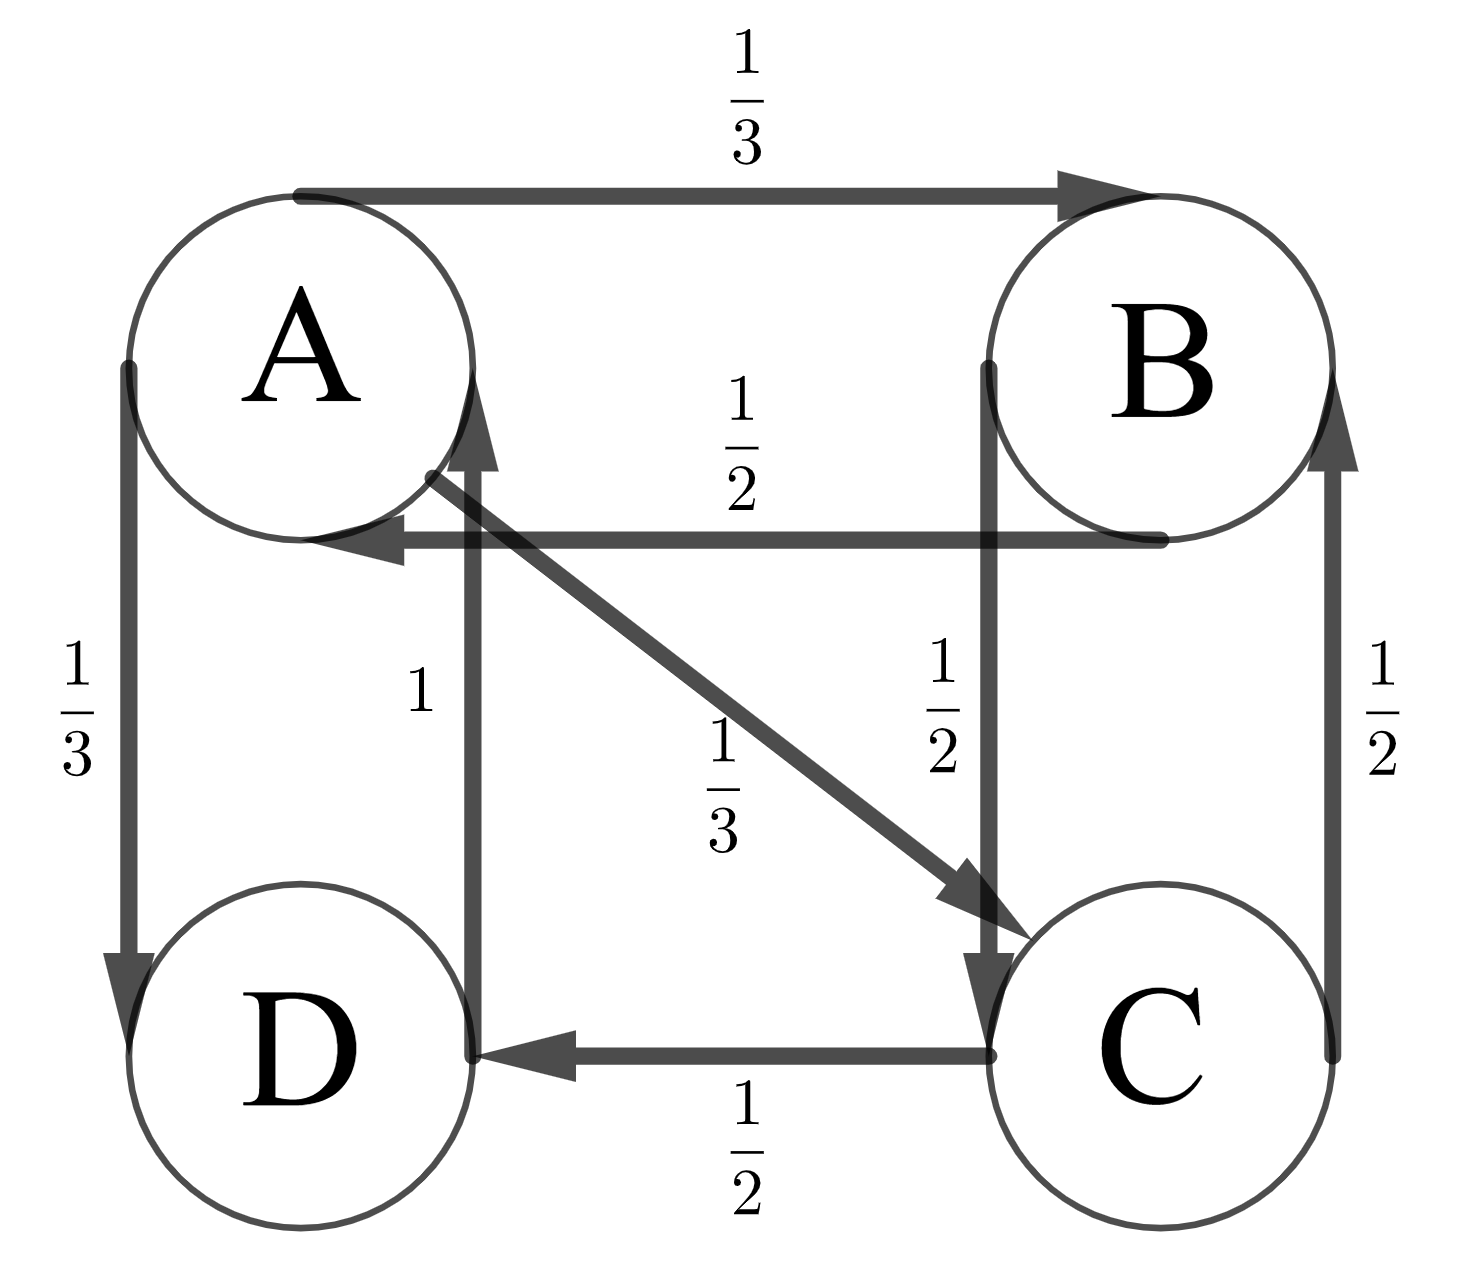
\includegraphics[scale=0.5]{figures/PageRank_exemple}
    \caption{Exemple de graphe pour l'illustration du calcul du PageRank.}
    \label{fig:PageRank_exemple}
\end{figure}

À partir du graphe de la figure~\ref{fig:PageRank_exemple}, la \gls{matricetransition} correspondante est donnée par :
\[
M =
\begin{bmatrix}
0   & \tfrac{1}{2} & 1 & 0 \\
\tfrac{1}{3} & 0 & 0 & \tfrac{1}{2} \\
\tfrac{1}{3} & 0 & 0 & \tfrac{1}{2} \\
\tfrac{1}{3} & \tfrac{1}{2} & 0 & 0
\end{bmatrix}.
\]

Chaque colonne de $M$ représente les probabilités de transition à partir d'une page donnée, et la matrice est \gls{stochastique}.

Si $v_i$ désigne la distribution des probabilités après $i$ itérations, alors :
\[
v_i = M v_{i-1}, \qquad v_i = M^i v_0,
\]
où $v_0$ est la distribution initiale uniforme :
\[
v_{0} =
\begin{bmatrix}
\tfrac{1}{4}\\[2pt]
\tfrac{1}{4}\\[2pt]
\tfrac{1}{4}\\[2pt]
\tfrac{1}{4}
\end{bmatrix}.
\]

\subsection{Calcul matriciel des premières itérations}

À partir de la matrice $M$ et du vecteur initial $v_0$, on obtient :

\paragraph{Première itération}
\[
v_{1} = Mv_{0} =
\begin{bmatrix}
\frac{3}{8}\\[2pt]
\frac{5}{24}\\[2pt]
\frac{5}{24}\\[2pt]
\frac{5}{24}
\end{bmatrix}.
\]

\paragraph{Itérations suivantes}
\[
v_{2} =
\begin{bmatrix}
\frac{5}{16}\\[2pt]
\frac{11}{48}\\[2pt]
\frac{11}{48}\\[2pt]
\frac{11}{48}
\end{bmatrix},
\qquad
v_{3} =
\begin{bmatrix}
\frac{11}{32}\\[2pt]
\frac{7}{32}\\[2pt]
\frac{7}{32}\\[2pt]
\frac{7}{32}
\end{bmatrix}.
\]

Après un nombre suffisant d'itérations, la suite $\{v_i\}$ converge vers la distribution stationnaire :
\[
v_{50} =
\begin{bmatrix}
\frac{1}{3}\\[2pt]
\frac{2}{9}\\[2pt]
\frac{2}{9}\\[2pt]
\frac{2}{9}
\end{bmatrix}.
\]
Cette distribution traduit la probabilité limite d'occurrence sur chaque page : le nœud $A$ concentre $\tfrac{1}{3}$ de la probabilité totale, tandis que $B$, $C$ et $D$ partagent chacun $\tfrac{2}{9}$.

\subsection{Exemple d'une première itération du PageRank}

Le graphe de la figure~\ref{fig:PageRank_exemple} peut être décrit par :
\[
\begin{cases}
A \to \{B, C, D\} \\[3pt]
B \to \{A, C\} \\[3pt]
C \to \{B, D\} \\[3pt]
D \to \{A\}
\end{cases}
\]

\paragraph{Initialisation}
\[
v_{(0)} = 
\begin{bmatrix}
0.25 & 0.25 & 0.25 & 0.25
\end{bmatrix}^{\top}.
\]

\paragraph{Distribution des contributions}
\[
\begin{aligned}
A &: 0.25/3 = 0.0833 \quad \text{vers } B, C, D,\\
B &: 0.25/2 = 0.125 \quad \text{vers } A, C,\\
C &: 0.25/2 = 0.125 \quad \text{vers } B, D,\\
D &: 0.25/1 = 0.25  \quad \text{vers } A.
\end{aligned}
\]

\paragraph{Somme des contributions reçues}
\[
\begin{aligned}
A &= 0.125 + 0.250 = 0.375,\\
B &= 0.0833 + 0.125 = 0.2083,\\
C &= 0.0833 + 0.125 = 0.2083,\\
D &= 0.0833 + 0.125 = 0.2083.
\end{aligned}
\]

\paragraph{Vecteur après une itération}
\[
v_{(1)} =
\begin{bmatrix}
0.375 & 0.2083 & 0.2083 & 0.2083
\end{bmatrix}^{\top}
\]

L'algorithme PageRank garantit la conservation de la masse de probabilité, la somme des composantes du vecteur restant égale à 1. En effet : $\sum\limits_i v^{(1)}_i = 1$.

Dans l'exemple présenté, le vecteur de probabilité stationnaire obtenu  au bout de 50 itérations est :

\[
v_{(50)} =
\begin{bmatrix}
\frac{1}{3} & \frac{2}{9} & \frac{2}{9} & \frac{2}{9}
\end{bmatrix}^{\top}
\]

Soit numériquement :

\[
v_{(50)} =
\begin{bmatrix}
0.3333 & 0.2222 & 0.2222 & 0.2222
\end{bmatrix}^{\top}
\]


La figure \ref{fig:PageRank_demo} illustre l'évolution du vecteur de probabilité associé au graphe de la figure \ref{fig:PageRank_exemple}.
Le calcul a été effectué avec un facteur d'amortissement ($d=1$), afin d'observer la convergence naturelle du processus de Markov sans composante de téléportation.
L'obtention de ce résultat s'est fait à l'aide de l'implémentation \gls{rdd} sans partitionnement, décrite dans la section \ref{subsection:RDD sans partitionnement}.

\begin{figure}[h]
    \centering
    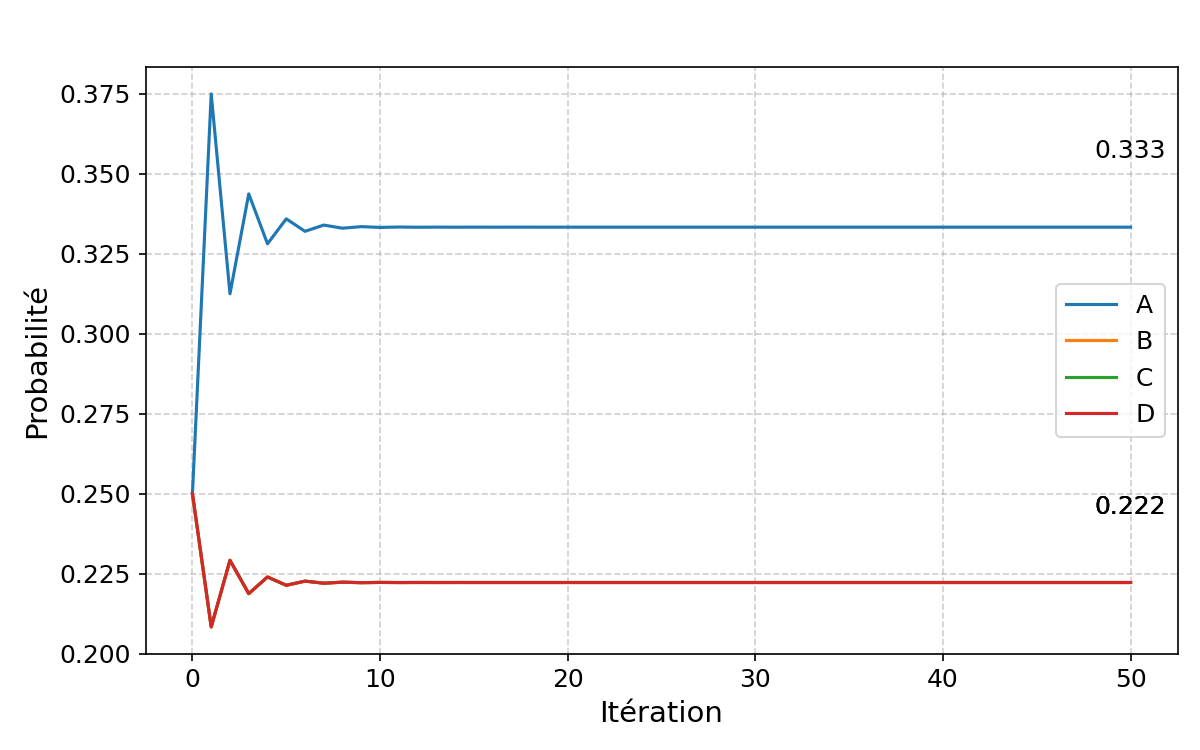
\includegraphics[width=0.8\linewidth]{figures/PageRank_evolution_demo}
    \caption{Convergence du graphe de la figure~\ref{fig:PageRank_exemple} sur 50 itérations, 
    obtenue à l'aide de l'implémentation RDD sans partitionnement\allowbreak{} de l'algorithme PageRank.}
    \label{fig:PageRank_demo}
\end{figure}

Cette étude de convergence met en évidence le comportement stationnaire du modèle \gls{pagerank}.

Abordons à présent l'implémentation en \gls{spark}, en détaillant les approches \gls{rdd} et \gls{dataframe} ainsi que les optimisations adoptées pour le traitement distribué.

\section{Implémentation Scala du PageRank}

L'implémentation de \gls{pagerank} a été réalisée en Scala au sein de l'environnement Apache \gls{spark}\footnote{L'ensemble de l'implémentation est disponible sur ce lien github : \url{https://github.com/auduvignac/pagerank-spark}}.
Ce choix repose sur la capacité de \gls{spark} à distribuer efficacement les calculs sur de larges volumes de données tout en offrant des abstractions adaptées à la manipulation de graphes.  
L'objectif de cette section est de détailler les différentes étapes de cette implémentation, depuis la structure générale du projet jusqu'à l'étude comparative des versions \gls{rdd} et \gls{dataframe}, avec et sans partitionnement explicite.

\subsection{Différences entre RDD et DataFrame}

Spark propose deux modèles de calcul principaux : les Resilient Distributed Dataset (\gls{rdd}) et les \glspl{dataframe}.  
Les \glspl{rdd} constituent l'abstraction fondamentale de \gls{spark}, représentant un ensemble distribué d'éléments partitionnés entre les nœuds du \gls{cluster}.
Ils offrent un contrôle fin sur les opérations et le partitionnement, mais nécessitent parfois une gestion explicite des transformations et des types de données.  

Les \glspl{dataframe}, quant à eux, reposent sur une abstraction de niveau supérieur inspirée du modèle relationnel.  
Ils permettent d'exprimer les transformations sous forme déclarative, optimisée par le moteur \gls{catalyst}.  
Bien que plus efficaces sur de nombreux cas d'usage, ils introduisent une couche d'optimisation automatique qui peut masquer certains détails de l'exécution.  

Ainsi, les expérimentations présentées dans ce travail comparent les performances et comportements des deux approches, dans un contexte identique de calcul du \gls{pagerank}.

\subsection{Structure du projet}

Le projet a été structuré de manière modulaire afin de faciliter la comparaison entre les différentes variantes d'implémentation.  
L'organisation générale se compose des éléments suivants :
\begin{itemize}
    \item \texttt{GraphRDD} et \texttt{GraphDF} : classes de représentation du graphe en \gls{rdd} et en \gls{dataframe} ;
    \item \texttt{PageRankRDD} et \texttt{PageRankDF} : implémentations respectives de l'algorithme \gls{pagerank} ;
    \item \texttt{Main} : point d'entrée du programme, permettant de sélectionner le mode d'exécution, le nombre de partitions et le fichier d'entrée ;
    \item \texttt{Benchmark} : module dédié à la collecte des métriques et à la comparaison des performances.
\end{itemize}

Pour garantir la cohérence des résultats sur les différents graphes, des tests unitaires ont été mis en place\footnote{\url{https://github.com/auduvignac/pagerank-spark/tree/main/src/test/scala/pagerank}} pour s'assurer du bon fonctionnement des classes utilisées et du bon fonctionnement de l'algorithme.

Pour chaque structure de données, l'implémentation de l'algorithme \gls{pagerank} s'articule autour d'une phase d'initialisation suivie d'une boucle itérative de calcul.

\subsection{Implémentation RDD sans partitionnement}\label{subsection:RDD sans partitionnement}

Cette première version s'appuie sur les mécanismes de partitionnement par défaut de \gls{spark}.  
Le graphe est chargé sous la forme d'un \gls{rdd} de paires \texttt{(page, liens\_sortants)}, sur lequel sont appliquées les transformations définies par l'algorithme \gls{pagerank}.  
Bien que simple à mettre en œuvre, cette approche ne tire pas pleinement parti de la localité des données, ce qui peut engendrer des coûts de communication importants lors des opérations de \texttt{join} et d'agrégation.

\paragraph{Initialisation}

En amont de la phase itérative, les structures nécessaires au calcul du \gls{pagerank} sont initialisées.
Le nombre total de pages $N$ est d'abord déterminé à partir de l'attribut \texttt{nNodes} de l'instance du graphe créé, puis les ensembles des nœuds et des liens sont chargés en mémoire distribuée et rendus persistants afin d'éviter leur rechargement à chaque itération.

\begin{lstlisting}[language=Scala]
val N: Double = graph.nNodes.toDouble
val allNodes: RDD[String] = graph.allNodes.persist(storage)
val links: RDD[(String, Seq[String])] = graph.links
\end{lstlisting}

Chaque nœud est ensuite associé à la liste de ses liens sortants ainsi qu'à son degré sortant $L(j)$.  
Les doublons sont supprimés afin de garantir une représentation unique des arêtes.

\begin{lstlisting}[language=Scala]
val outMap: RDD[(String, (Int, Seq[String]))] = links
  .reduceByKey(_ ++ _)
  .mapValues(_.distinct)
  .mapValues(outs => (outs.size, outs))
\end{lstlisting}

Les nœuds dépourvus de liens sortants (\glspl{danglingnode}) sont ajoutés à la structure, avec un degré nul et une liste vide, afin de conserver un graphe complet et cohérent.

\begin{lstlisting}[language=Scala]
val nodesWithOut: RDD[(String, (Int, Seq[String]))] = allNodes
  .map(nodeId => (nodeId, (0, Seq.empty[String])))
  .leftOuterJoin(outMap)
  .mapValues {
    case ((_, _), Some((deg, outs))) => (deg, outs)
    case _                           => (0, Seq.empty[String])
  }
  .persist(storage)
\end{lstlisting}

Enfin, le vecteur des rangs $v_0$ est initialisé de manière uniforme :
\[
v_0 = \left[ \frac{1}{N}, \frac{1}{N}, \ldots, \frac{1}{N} \right]^{\top}
\]
ce qui correspond à une probabilité égale pour chaque page d'être visitée au départ.

\begin{lstlisting}[language=Scala]
var ranks: RDD[(String, Double)] = allNodes
  .map(n => (n, 1.0 / N))
  .persist(storage)
\end{lstlisting}

\paragraph{Boucle itérative (fonction \texttt{oneStep}) :}

La fonction \texttt{oneStep} réalise une itération complète du calcul du \gls{pagerank}, selon le principe de mise à jour :
\[
v_{i+1} = M  v_i.
\]
Elle est appelée successivement jusqu'à atteindre le nombre maximal d'itérations défini dans la configuration du benchmark\footnote{Certaines implémentations interrompent le calcul dès que la convergence est atteinte. Dans le présent travail, l'objectif a été de se concentrer exclusivement sur les temps de traitement générés par les approches \gls{rdd} et \gls{dataframe}, indépendamment du critère de convergence.}.

\begin{lstlisting}[language=Scala]
def oneStep(
    ranks: RDD[(String, Double)],
    nodesWithOut: RDD[(String, (Int, Seq[String]))],
    allNodes: RDD[String],
    N: Double,
    damping: Double = 1.0,
    debug: Boolean = false,
    logger: Logger
): RDD[(String, Double)] = {
\end{lstlisting}

\textbf{Calcul de la masse des \glspl{danglingnode}}  
Les pages sans lien sortant transfèrent leur poids total à la masse globale \texttt{danglingMass}, qui sera redistribuée uniformément sur l'ensemble du graphe.

\begin{lstlisting}[language=Scala]
val danglingMass = nodesWithOut.join(ranks)
  .filter { case (_, ((deg, _), _)) => deg == 0 }
  .map { case (_, ((_, _), r)) => r }
  .sum()
\end{lstlisting}

\textbf{Calcul des contributions des nœuds \textit{non-dangling}}  
Les pages disposant de liens sortants distribuent leur score proportionnellement à leur degré sortant.  
Chaque destination $d$ reçoit une contribution $PR(j) / L(j)$ provenant de la page $j$.

\begin{lstlisting}[language=Scala]
val contribs = nodesWithOut.join(ranks)
  .flatMap { case (_, ((deg, outs), r)) =>
    if (deg == 0) Iterator.empty
    else outs.iterator.map(d => (d, r / deg))
  }
  .reduceByKey(_ + _)
\end{lstlisting}

\textbf{Calcul du terme uniforme et redistribution de la masse des \glspl{danglingnode}}  
Le facteur d'amortissement $d$ (ou \textit{damping factor}) est appliqué afin de simuler le comportement d'un internaute aléatoire, conformément au modèle de navigation décrit en section~\ref{eq:pagerank-dangling}.

\begin{lstlisting}[language=Scala]
val base = ((1.0 - damping) / N) + (damping * danglingMass / N)
\end{lstlisting}

\textbf{Calcul des nouveaux rangs}  
Chaque page reçoit à la fois le terme uniforme et les contributions des pages qui pointent vers elle.  
L'opération \texttt{leftOuterJoin} garantit l'inclusion de toutes les pages, y compris celles sans lien entrant.

\begin{lstlisting}[language=Scala]
val newRanks = allNodes
  .map(id => (id, base))
  .leftOuterJoin(contribs)
  .mapValues { case (b, cOpt) => b + damping * cOpt.getOrElse(0.0) }
\end{lstlisting}

\textbf{Normalisation du vecteur de rangs}  
La somme totale des rangs est recalculée afin de garantir la propriété de normalisation :
\[
\sum_i PR(i) = 1.
\]
Cette étape assure que le vecteur de rangs demeure une distribution de probabilité valide.

\begin{lstlisting}[language=Scala]
val sumRanks = newRanks.values.sum()
val normalizedRanks = newRanks.mapValues(_ / sumRanks)
normalizedRanks
\end{lstlisting}

\paragraph{Analyse}

Cette première implémentation met directement en œuvre la formulation mathématique du \gls{pagerank}.  
Elle présente l'avantage de la simplicité et d'une lecture claire du flux de calcul distribué.  
Cependant, en l'absence de partitionnement explicite, les transformations comme \texttt{join} ou \texttt{reduceByKey} entraînent des échanges de données fréquents entre les nœuds du \gls{cluster}, ce qui limite la scalabilité sur des graphes de grande taille.

Dans la section suivante, une version optimisée introduit un partitionnement cohérent des \glspl{rdd}, afin de réduire les coûts de communication et d'améliorer la localité des calculs.

\subsection{Implémentation RDD avec partitionnement}

Cette seconde version améliore la précédente en introduisant un partitionnement explicite des \glspl{rdd}.  
L'objectif est de minimiser les transferts de données entre les nœuds du \gls{cluster} lors des opérations de \texttt{join} et de \texttt{reduceByKey}, qui constituent les étapes les plus coûteuses du calcul du \gls{pagerank}.  

\paragraph{Principe général}

Alors que la version précédente reposait sur le partitionnement implicite de Spark, cette implémentation définit un partitionneur explicite de type \texttt{HashPartitioner}.  
Celui-ci garantit que les \glspl{rdd} manipulés (\texttt{ranks}, \texttt{nodesWithOut}, \texttt{outMap}) sont répartis selon la même logique de hachage des clefs, ce qui permet aux jointures successives de s'exécuter localement, sans provoquer de \textit{shuffle}.

\begin{lstlisting}[language=Scala]
val P = new HashPartitioner(
  if (numParts > 0) numParts
  else sc.defaultParallelism * 2
)
\end{lstlisting}

Le \og partitionneur \fg{} est ensuite appliqué systématiquement à toutes les structures manipulées :
\begin{itemize}
  \item \texttt{outMap} et \texttt{nodesWithOut} sont construits avec le \og partitionneur \fg{} $P$ ;
  \item le vecteur \texttt{ranks} est également partitionné selon $P$ ;
  \item toutes les jointures ultérieures (\texttt{join}, \texttt{leftOuterJoin}) bénéficient ainsi d'une co-localisation des données.
\end{itemize}

Cette homogénéité de partitionnement permet d'éviter le déclenchement automatique de \texttt{shuffle}, l'une des principales sources de surcharge lors des traitements distribués sur des graphes volumineux.

\paragraph{Différences principales avec la version sans partitionnement}

L'algorithme implémenté dans la méthode \texttt{oneStep} conserve la même logique computationnelle que celle décrite dans la section précédente : calcul de la masse des \glspl{danglingnode}, distribution des contributions, application du facteur d'amortissement et normalisation finale.  
Cependant, plusieurs optimisations structurelles sont introduites :

\begin{enumerate}
    \item \textbf{Jointure unique et persistée :}  
    Les informations des nœuds et des rangs sont réunies en une seule jointure stockée en mémoire :
    \begin{lstlisting}[language=Scala]
val joined = nodesWithOut.join(ranks).persist(storage)
    \end{lstlisting}
    Cela permet de réutiliser la même structure à la fois pour le calcul de la masse des \glspl{danglingnode} et pour celui des contributions, réduisant ainsi le coût global de calcul.

    \item \textbf{Utilisation du \og partitionneur \fg{} dans les agrégations :}  
    Les réductions sont désormais exécutées avec le \og partitionneur \fg{} $P$, ce qui garantit la localité des opérations :
    \begin{lstlisting}[language=Scala]
.reduceByKey(partitioner, _ + _)
    \end{lstlisting}
    Cette optimisation élimine les transferts inter-partitions inutiles lors de l'agrégation des contributions.

    \item \textbf{Évaluation locale des sommes partielles :}  
    La somme totale des rangs est calculée par partition avant réduction globale :
    \begin{lstlisting}[language=Scala]
val sumRanks = newRanks.mapPartitions(it => Iterator(it.map(_._2).sum)).sum()
    \end{lstlisting}
    Ce procédé limite les échanges de données et exploite efficacement le parallélisme offert par les exécuteurs Spark.

    \item \textbf{Structures compactes et typées :}  
    Les liens sortants sont stockés sous forme de \texttt{Array[String]} plutôt que de \texttt{Seq[String]}, permettant un accès séquentiel plus rapide et une empreinte mémoire réduite sur le \gls{cluster}.
\end{enumerate}

\paragraph{Synthèse comparative}

Le tableau~\ref{tab:rdd-vs-rddpart} résume les principales différences entre les deux implémentations.

\begin{table}[H]
\centering
\caption{Comparaison entre les implémentations RDD sans et avec partitionnement}
\label{tab:rdd-vs-rddpart}
\renewcommand{\arraystretch}{1.2}
\begin{tabularx}{\linewidth}{|>{\raggedright\arraybackslash}p{3cm}|X|X|}
\hline
\textbf{Aspect} & \textbf{RDD sans partitionnement} & \textbf{RDD avec partitionnement} \\
\hline
Partitionnement & Automatique (par Spark) & \texttt{HashPartitioner} explicite appliqué à tous les RDD \\
\hline
Jointures & Chaque \texttt{join} déclenche un \textit{shuffle} & Jointures locales (même partitionneur) \\
\hline
Persistance & Limitée aux RDD principaux & Persistences intermédiaires pour éviter recomputation \\
\hline
Type de structure & \texttt{Seq[String]} & \texttt{Array[String]} (plus compact et rapide) \\
\hline
Calcul des sommes & Réduction globale (\texttt{sum}) & Réduction locale par partition (\texttt{mapPartitions}) \\
\hline
Coût réseau & Élevé (multiples transferts) & Réduit (localité des données) \\
\hline
Performance & Simplicité d'exécution, bonne lisibilité & Optimisée pour la scalabilité sur grands graphes \\
\hline
\end{tabularx}
\end{table}

\paragraph{Analyse}

L'ajout d'un \og partitionneur \fg{} cohérent entre les \glspl{rdd} constitue une optimisation majeure dans le calcul du \gls{pagerank}.
Il permet d'exploiter la localité des données, de réduire les coûts de communication entre les exécuteurs et d'améliorer la reproductibilité des performances sur des graphes massifs.  

Cette approche se rapproche d'une configuration typique de production, où le partitionnement et la persistance des structures sont ajustés pour garantir un compromis optimal entre consommation mémoire et débit de traitement.  
La section suivante présente la transposition de cette logique à l'approche \gls{dataframe}, exploitant cette fois le moteur d'exécution \gls{catalyst}.

\subsection{Implémentation DataFrame sans partitionnement}
 
Cette version s'appuie sur les opérations de haut niveau du moteur \gls{catalyst}, qui optimise automatiquement les plans d'exécution grâce à un analyseur logique et physique.  
L'objectif est d'exploiter les capacités de projection, d'agrégation et de jointure de \gls{dataframe} tout en conservant la logique mathématique décrite précédemment.

\paragraph{Initialisation des structures de données}

Les différentes étapes de préparation consistent à structurer le graphe sous forme de tables relationnelles distribuées, en calculant les degrés sortants et en identifiant les \glspl{danglingnode}.

\begin{lstlisting}[language=Scala]
val N: Double = graph.nNodes.toDouble

val edges = graph.links
  .filter(col("outlink").isNotNull)
  .select(col("page").as("src"), col("outlink").as("dest"))
  .distinct()
  .persist(storage)
\end{lstlisting}

La table \texttt{edges} représente l'ensemble des arêtes du graphe, c'est-à-dire les transitions $(u, v)$ entre pages.  
Les nœuds sont ensuite extraits à partir des colonnes \texttt{src} et \texttt{dest} :

\begin{lstlisting}[language=Scala]
val nodes = edges.select(col("src").as("id"))
  .union(edges.select(col("dest").as("id")))
  .distinct()
  .persist(storage)
\end{lstlisting}

Le degré sortant de chaque page est obtenu par un \texttt{groupBy} et un \texttt{count} :

\begin{lstlisting}[language=Scala]
val outdeg = edges
  .groupBy(col("src"))
  .agg(count(lit(1)).as("outdeg"))
  .withColumnRenamed("src", "id")
  .persist(storage)
\end{lstlisting}

Les nœuds sont ensuite enrichis avec leur degré sortant, les nœuds absents de \texttt{outdeg} étant considérés comme \glspl{danglingnode} ($L(j) = 0$) :

\begin{lstlisting}[language=Scala]
val nodesWithDeg = nodes
  .join(outdeg, Seq("id"), "left")
  .na.fill(0, Seq("outdeg"))
  .persist(storage)
\end{lstlisting}

L'ensemble des pages sans lien sortant est ensuite identifié :

\begin{lstlisting}[language=Scala]
val danglingIds = nodesWithDeg
  .filter(col("outdeg") === 0)
  .select(col("id"))
  .persist(storage)
\end{lstlisting}

Enfin, le vecteur initial des rangs est uniformément réparti sur toutes les pages :

\[
v_0 = \left[ \frac{1}{N}, \frac{1}{N}, \ldots, \frac{1}{N} \right]^{\top}
\]

\begin{lstlisting}[language=Scala]
var ranks = nodes
  .withColumn("rank", lit(1.0 / N))
  .persist(storage)
  .localCheckpoint(eager = true)
\end{lstlisting}

\paragraph{Itération principale (fonction \texttt{oneStep})}

La fonction \texttt{oneStep} reproduit la même logique mathématique que celle présentée pour les \glspl{rdd}, mais implémentée ici à l'aide d'opérations SQL distribuées.  

\begin{lstlisting}[language=Scala]
def oneStep(
    ranks: DataFrame,
    edges: DataFrame,
    nodes: DataFrame,
    outdegPos: DataFrame,
    danglingIds: DataFrame,
    N: Double,
    damping: Double = 1.0,
    storage: StorageLevel = StorageLevel.MEMORY_ONLY,
    debug: Boolean = false,
    logger: Logger
)(implicit spark: SparkSession): DataFrame = {
\end{lstlisting}

\textbf{Masse des \glspl{danglingnode}}  
Les pages sans liens sortants sont identifiées et leur masse de probabilité totale est sommée à l'aide d'une jointure en mode \texttt{left\_semi} :

\begin{lstlisting}[language=Scala]
val danglingMass: Double =
  ranks.join(danglingIds, Seq("id"), "left_semi")
    .select(col("rank"))
    .rdd.map(_.getDouble(0)).sum()
\end{lstlisting}

Cette étape correspond au calcul de $S = \sum\limits_{u \in D} PR(u)$ dans la formule~\eqref{eq:pagerank-dangling}.

\textbf{Calcul des contributions}  
Chaque page \textit{non-dangling} distribue sa probabilité à ses destinations.  
L'opération s'effectue via deux jointures successives : \texttt{edges}~$\leftrightarrow$~\texttt{ranks} et \texttt{edges}~$\leftrightarrow$~\texttt{outdegPos}, suivie d'une agrégation par \texttt{dest} :

\begin{lstlisting}[language=Scala]
val contribs = edges
  .join(
    ranks.select(col("id").as("src"), col("rank").as("rank_src")),
    Seq("src"), "inner"
  )
  .join(outdegPos, Seq("src"), "inner")
  .withColumn("contrib", col("rank_src") / col("outdeg"))
  .groupBy(col("dest").as("id"))
  .agg(sum(col("contrib")).as("sumContrib"))
  .persist(storage)
\end{lstlisting}

\textbf{Application du facteur d'amortissement}  
Le facteur $d$ est appliqué à la fois sur les contributions et sur le terme uniforme $\tfrac{1 - d}{N}$, auquel s'ajoute la redistribution de la masse des \glspl{danglingnode} :

\[
PR(i) = \frac{1 - d}{N} + d \left( \sum_{j \in M(i)} \frac{PR(j)}{L(j)} + \frac{S}{N} \right).
\]

\begin{lstlisting}[language=Scala]
val base = ((1.0 - damping) / N) + (damping * danglingMass / N)
\end{lstlisting}

Les nouveaux rangs sont calculés en effectuant une jointure externe entre les nœuds et leurs contributions :

\begin{lstlisting}[language=Scala]
val newRanks = nodes
  .join(contribs, Seq("id"), "left")
  .select(
    col("id"),
    (lit(base) + lit(damping) * coalesce(col("sumContrib"), lit(0.0))).as("rank")
  )
  .persist(storage)
\end{lstlisting}

\textbf{Normalisation du vecteur de rangs}  
Comme dans la version \gls{rdd}, la somme totale des rangs est ramenée à 1 pour assurer la cohérence probabiliste.

\begin{lstlisting}[language=Scala]
val sumRanks = newRanks.select(col("rank")).rdd.mapPartitions(it =>
  Iterator(it.map(_.getDouble(0)).sum)
).sum()

val normalizedRanks = newRanks
  .withColumn("rank", col("rank") / lit(sumRanks))
  .localCheckpoint(eager = true)
\end{lstlisting}

\paragraph{Analyse comparative}

L'approche \gls{dataframe} offre une abstraction plus déclarative que les \glspl{rdd}.
Elle repose sur des transformations logiques optimisées par le moteur \gls{catalyst}, qui choisit automatiquement les stratégies de jointure et les plans physiques les plus efficaces.  

Cependant, en l'absence de partitionnement explicite, les jointures entre \texttt{edges}, \texttt{ranks} et \texttt{outdeg} entraînent des opérations de \textit{shuffle} réseau analogues à celles observées dans la version \gls{rdd} non partitionnée.  
Par ailleurs, cette approche permet une formulation plus compacte, compatible avec les \gls{api} SQL et les extensions du moteur \gls{dataframe}.

La section suivante présente la version partitionnée, qui applique les principes de co-localisation des données déjà explorés dans le cas des \glspl{rdd}.

\subsection{Implémentation DataFrame avec partitionnement}

Cette implémentation vise à améliorer la localité des opérations et à réduire les coûts de \textit{shuffle} réseau, tout en bénéficiant des optimisations du moteur d'exécution \gls{catalyst}.  

Contrairement à la version précédente, où le partitionnement était implicite, cette implémentation répartit explicitement les \glspl{dataframe} selon des colonnes clefs (\texttt{src} ou \texttt{id}), afin de garantir la co-localisation des données lors des jointures successives.

\paragraph{Initialisation et partitionnement}

Un nombre de partitions $p$ est défini à partir du degré de parallélisme du \gls{cluster} :

\begin{lstlisting}[language=Scala]
val p = if (numParts > 0) numParts else spark.sparkContext.defaultParallelism * 2
\end{lstlisting}

Toutes les structures de base (\texttt{edges}, \texttt{nodes}, \texttt{outdeg}, \texttt{ranks}) sont ensuite explicitement réparties sur ces partitions.

\begin{itemize}
  \item Les arêtes sont partitionnées par plage de valeurs de la colonne \texttt{src} :
  \begin{lstlisting}[language=Scala]
.repartitionByRange(p, col("src"))
  \end{lstlisting}
  ce qui assure que toutes les arêtes partageant la même source sont regroupées sur la même partition.

  \item Les nœuds et le vecteur de rangs sont également répartis par \texttt{id}, garantissant un alignement parfait entre les structures :
  \begin{lstlisting}[language=Scala]
.repartition(p, col("id"))
  \end{lstlisting}

  \item Le degré sortant (\texttt{outdeg}) est calculé localement sur chaque partition, puis répartitionné sur la clef \texttt{id} afin de limiter les échanges de données entre partitions.
\end{itemize}

Ainsi, les jointures successives entre \texttt{edges}, \texttt{ranks} et \texttt{outdeg} peuvent être effectuées localement sans déclencher de \textit{shuffle} global.

\paragraph{Itération principale (fonction \texttt{oneStep}) :}

La logique de calcul reste identique à celle de la version non partitionnée :  
calcul de la masse des \glspl{danglingnode}, distribution des contributions, application du facteur d'amortissement et normalisation du vecteur des rangs.  

Cependant, plusieurs différences notables ont pour vocation à renforcer l'efficacité de cette implémentation :

\begin{enumerate}
  \item \textbf{Optimisation du calcul de la masse des \glspl{danglingnode}}  
  Le calcul de la masse totale est effectué via l'\gls{api} \gls{rdd}, afin d'éviter la matérialisation complète du plan logique \gls{catalyst} :
  \begin{lstlisting}[language=Scala]
val danglingMass: Double =
  ranks.join(danglingIds, Seq("id"), "left_semi")
    .select(col("rank"))
    .rdd.map(_.getDouble(0)).sum()
  \end{lstlisting}
  Cette approche combine la simplicité du modèle \gls{dataframe} avec la performance du modèle bas-niveau \texttt{RDD.sum()}.

  \item \textbf{Jointures locales et partitionnées}  
  Toutes les jointures sont réalisées sur des colonnes déjà alignées et partitionnées, évitant ainsi la redistribution des données :
  \begin{lstlisting}[language=Scala]
.join(outdegPos, Seq("src"), "inner")
  \end{lstlisting}
  Contrairement à la version non partitionnée, aucune réorganisation globale du plan n'est nécessaire.

  \item \textbf{Calcul distribué des contributions}  
  Les contributions sont regroupées par clef locale grâce à \texttt{groupBy(col("dest"))}, puis agrégées par somme.  
  Chaque partition traite ainsi son sous-ensemble du graphe en quasi-autonomie, réduisant la charge sur le moteur d'exécution \gls{catalyst}.

  \item \textbf{Normalisation locale}  
  La somme totale des rangs est obtenue via un calcul distribué par partition :
  \begin{lstlisting}[language=Scala]
val sumRanks = newRanks.select(col("rank")).rdd
  .mapPartitions(it => Iterator(it.map(_.getDouble(0)).sum))
  .sum()
  \end{lstlisting}
  Cette technique réduit considérablement le volume des données agrégées globalement.
\end{enumerate}

\paragraph{Analyse comparative}

Le tableau~\ref{tab:df-vs-dfpart} résume les différences principales entre les versions \gls{dataframe} sans et avec partitionnement.

\begin{table}[H]
\centering
\caption{Comparaison entre les implémentations \gls{dataframe} sans et avec partitionnement}
\label{tab:df-vs-dfpart}
\renewcommand{\arraystretch}{1.2}
\begin{tabularx}{\linewidth}{|>{\raggedright\arraybackslash}p{3cm}|X|X|}
\hline
\textbf{Aspect} & \textbf{DF sans partitionnement} & \textbf{DF avec partitionnement} \\
\hline
Partitionnement & Automatique (Catalyst) & Explicite via \texttt{repartitionByRange} ou \texttt{repartition(p, col("id"))} \\
\hline
Jointures & Multiples \textit{shuffle} réseau & Jointures locales entre partitions alignées \\
\hline
Plan d'exécution & Recalcul complet à chaque itération & Réutilisation locale des partitions et persistance \\
\hline
Calcul des sommes & Global via Catalyst & Local via \texttt{RDD.mapPartitions} \\
\hline
Coût réseau & Élevé (redistribution implicite) & Réduit (co-localisation explicite des données) \\
\hline
Performance & Dépendante du plan Catalyst & Optimisée pour la scalabilité et la localité \\
\hline
Lisibilité du code & Plus concise et déclarative & Plus technique, mais mieux contrôlée \\
\hline
\end{tabularx}
\end{table}

\paragraph{Synthèse}

Le passage d'une approche \gls{dataframe} non partitionnée à une version partitionnée permet d'exploiter plus efficacement la parallélisation intra-cluster.  
En combinant la co-localisation des données avec les optimisations automatiques du moteur \gls{catalyst}, cette version constitue un compromis performant entre le modèle déclaratif de Spark SQL et la maîtrise fine du traitement distribué.  

Elle se rapproche ainsi du comportement de la version \gls{rdd} partitionnée tout en conservant les avantages analytiques et expressifs du modèle \gls{dataframe}.

Les quatre implémentations présentées traduisent des choix de modélisation et d'optimisation distincts du calcul du \gls{pagerank}.  
Chacune d'elle met en évidence un compromis entre simplicité de mise en œuvre, maîtrise du partitionnement, et efficacité d'exécution au sein du \gls{cluster}.

Afin d'évaluer de manière objective leurs performances respectives, une succession de tests a été réalisée sur différents graphes représentatifs.
L'objectif est d'analyser l'impact du modèle de données et des stratégies de partitionnement sur les temps d'exécution, la charge du \textit{garbage collector}, et la consommation des ressources mémoire.

Pour assurer une comparaison équitable entre implémentation et taille de graphe, la configuration \texttt{Spark} utilisée est la même pour chaque exécution.

\clearpage

\section{Configuration \gls{spark} utilisée pour les mesures}

L'ensemble des expérimentations a été réalisé à l'aide de la configuration suivante, appliquée lors de l'exécution du programme via la commande \texttt{spark-submit} sur le \gls{cluster} Lamsade :

\begin{lstlisting}
spark-submit \
  --class pagerank.Main \
  --deploy-mode client \
  --executor-cores 4 \
  --num-executors 8 \
  --executor-memory 10G \
  --driver-memory 6G \
  --conf "spark.serializer=org.apache.spark.serializer.KryoSerializer" \
  --conf "spark.kryoserializer.buffer.max=512m" \
  --conf "spark.default.parallelism=48" \
  --conf "spark.sql.shuffle.partitions=48" \
  --conf "spark.memory.fraction=0.8" \
  --conf "spark.memory.offHeap.enabled=true" \
  --conf "spark.memory.offHeap.size=4g" \
  --conf "spark.speculation=false" \
  --conf "spark.locality.wait=0" \
  --conf "spark.shuffle.compress=true" \
  --conf "spark.shuffle.spill.compress=true" \
  --conf "spark.shuffle.file.buffer=256k" \
  --conf "spark.reducer.maxSizeInFlight=256m" \
  --conf "spark.rdd.compress=true" \
  --conf "spark.io.compression.codec=lz4" \
  --conf "spark.sql.adaptive.enabled=false" \
  --conf "spark.executor.memoryOverhead=2G" \
  --conf "spark.executor.extraJavaOptions=-XX:+UseG1GC -XX:+UseStringDeduplication"
\end{lstlisting}

Cette configuration vise à garantir un compromis entre la stabilité, la reproductibilité et la performance du calcul distribué.  
Le choix de \texttt{8} exécuteurs dotés chacun de \texttt{4} cœurs et de \texttt{10~Go} de mémoire permet de répartir efficacement les partitions sur le \gls{cluster} tout en évitant la saturation mémoire.  
L'utilisation du sérialiseur \texttt{Kryo} améliore la vitesse de transfert des objets entre les nœuds, réduisant ainsi la latence du \textit{shuffle}.

Les paramètres de mémoire hors tas (\texttt{offHeap}) et la compression \texttt{LZ4} contribuent à limiter la pression sur le \textit{garbage collector}, particulièrement sensible lors du traitement des grands graphes.  
Le choix du collecteur \texttt{G1GC} associé à l'option \texttt{UseStringDeduplication} favorise une gestion plus efficace des chaînes de caractères et une meilleure stabilité du temps d'exécution.

Enfin, la désactivation de l'exécution adaptative (\texttt{spark.sql.adaptive.enabled=false}) garantit la comparabilité entre les différentes structures de calcul (\gls{rdd} et \gls{dataframe}) en évitant que Spark ne modifie dynamiquement le plan d'exécution au cours du \textit{benchmark}.

Cette configuration influe directement sur les performances observées dans les résultats décrits dans ce rapport.
Le paramètre \texttt{spark.default.parallelism=48} impose un degré de parallélisme constant entre les différentes exécutions, garantissant une répartition homogène des tâches sur l'ensemble des exécuteurs.  
Ce réglage favorise une utilisation efficace des ressources de calcul, tout en limitant les déséquilibres de charge susceptibles de fausser les comparaisons entre implémentations.

Les paramètres liés à la mémoire jouent également un rôle déterminant.  
L'activation de la mémoire hors tas (\texttt{offHeap}) et la définition d'une fraction mémoire élevée (\texttt{spark.memory.fraction=0.8}) permettent de réduire les accès disques et de mieux contrôler la pression exercée sur le \textit{garbage collector}.  
Ces ajustements se traduisent par une diminution du temps consacré au nettoyage mémoire, notamment pour les grands graphes tels que \texttt{wiki-pt.txt} et \texttt{wiki-fr.txt}.

La désactivation de la spéculation (\texttt{spark.speculation=false}) empêche la relance de tâches supposées lentes, évitant ainsi les fluctuations de performance entre itérations successives.  
De même, la compression des échanges (\texttt{spark.shuffle.compress=true}) et la limitation de la taille des transferts inter-nœuds (\texttt{spark.reducer.maxSizeInFlight=256m}) réduisent le coût global des opérations de \textit{shuffle}, particulièrement sollicitées lors des agrégations dans les implémentations \gls{rdd}.

Enfin, le choix du collecteur \texttt{G1GC}, associé à la déduplication des chaînes de caractères, assure une gestion plus stable de la mémoire lors du calcul du \gls{pagerank}.  
Cette configuration favorise une progression plus régulière du calcul itératif, en particulier pour les graphes de grande taille où les volumes de données échangées entre partitions sont significatifs.

De plus, le paramètre de stockage a été fixé à \texttt{MEMORY\_AND\_DISK\_SER}, tandis que le facteur d'amortissement a été défini à 
0,85.

La section suivante présente les résultats expérimentaux issus de ces exécutions, ainsi que les visualisations associées, permettant de comparer quantitativement le comportement de chaque approche.

\section{Analyse quantitative des temps d'exécution}

La première phase d'analyse des performances de chaque implémentation s'est limitée à l'affichage successif du temps global associé à chaque graphe.

Le tableau \ref{tab:benchmark_times} présente les temps d'exécution selon la taille des graphes et la méthode utilisée avec 10 itérations.

\begin{table}[ht]
\centering
\caption{Temps d'exécution du \gls{pagerank} selon la taille des graphes et la méthode utilisée (10 itérations).}
\label{tab:benchmark_times}
\renewcommand{\arraystretch}{1.2}
\setlength{\tabcolsep}{4pt}
\begin{tabular}{|l|r|r|l|r|}
\hline
\textbf{Graphe} & \textbf{Nœuds} & \textbf{Arêtes} & \textbf{Méthode} & \textbf{Temps (s)} \\
\hline
\multirow{4}{*}{wiki-chti.txt}
 & 15489 & 40124 & RDD & 75.21 \\
 &  &  & RDD Partitionné & 59.88 \\
 &  &  & DF & 103.25 \\
 &  &  & DF Partitionné & 99.81 \\
\hline
\multirow{4}{*}{wiki-breton.txt}
 & 379763 & 1408847 & RDD & 242.17 \\
 &  &  & RDD Partitionné & 223.82 \\
 &  &  & DF & 176.15 \\
 &  &  & DF Partitionné & 172.99 \\
\hline
\multirow{4}{*}{wiki-basque.txt}
 & 761282 & 4616203 & RDD & 338.33 \\
 &  &  & RDD Partitionné & 379.41 \\
 &  &  & DF & 284.74 \\
 &  &  & DF Partitionné & 304.33 \\
\hline
\multirow{4}{*}{wiki-pt.txt}
 & 3765539 & 31571024 & RDD & 4067.32 \\
 &  &  & RDD Partitionné & 801.45 \\
 &  &  & DF & 597.40 \\
 &  &  & DF Partitionné & 576.56 \\
\hline
\multirow{4}{*}{wiki-fr.txt}
 & 6740183 & 80920486 & RDD & 4831.34 \\
 &  &  & RDD Partitionné & 2201.41 \\
 &  &  & DF & 1348.86 \\
 &  &  & DF Partitionné & 1884.48 \\
\hline
\end{tabular}
\end{table}

En supplément du tableau \ref{tab:benchmark_times}, la figure \ref{fig:benchmark_times} regroupe deux visualisations complémentaires :
\begin{itemize}
    \item la figure~\ref{fig:benchmark_times_evolution} montrant l'évolution des temps d'exécution en fonction de la taille des graphes ;
    \item la figure~\ref{fig:benchmark_times_bar} comparant directement les quatre implémentations sur un même graphique synthétique.
\end{itemize}

\begin{figure}[ht]
    \centering

    \subfloat[\textbf{Évolution des temps d'exécution selon la taille des graphes.}\label{fig:benchmark_times_evolution}]{
        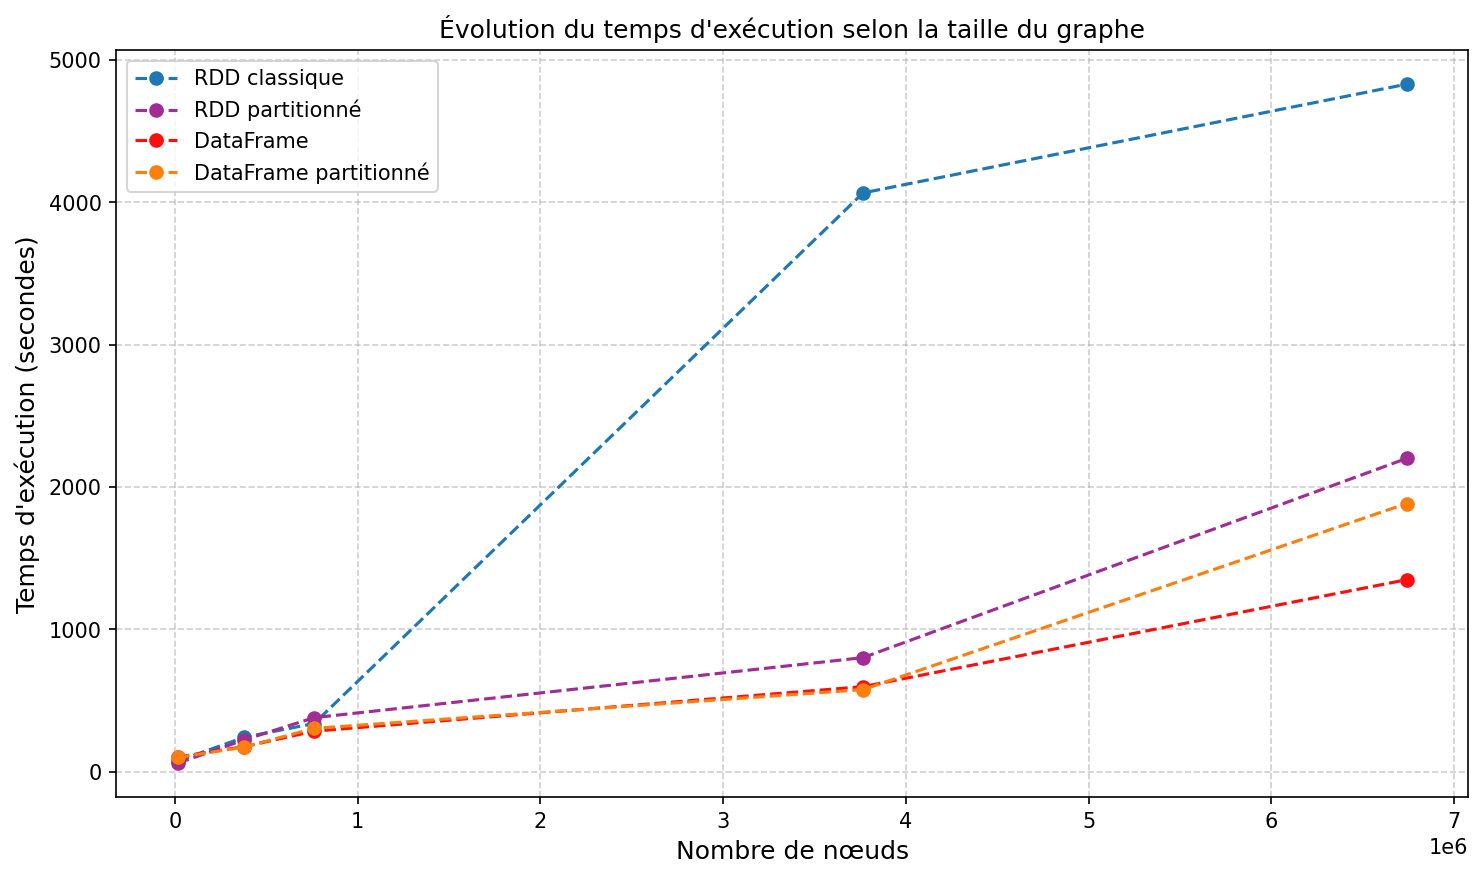
\includegraphics[width=0.45\textwidth]{figures/benchmark_times_evolution}
    }

    \vspace{0.8em}


    \subfloat[\textbf{Comparaison directe des temps d'exécution par implémentation (diagramme en barres).}\label{fig:benchmark_times_bar}]{
        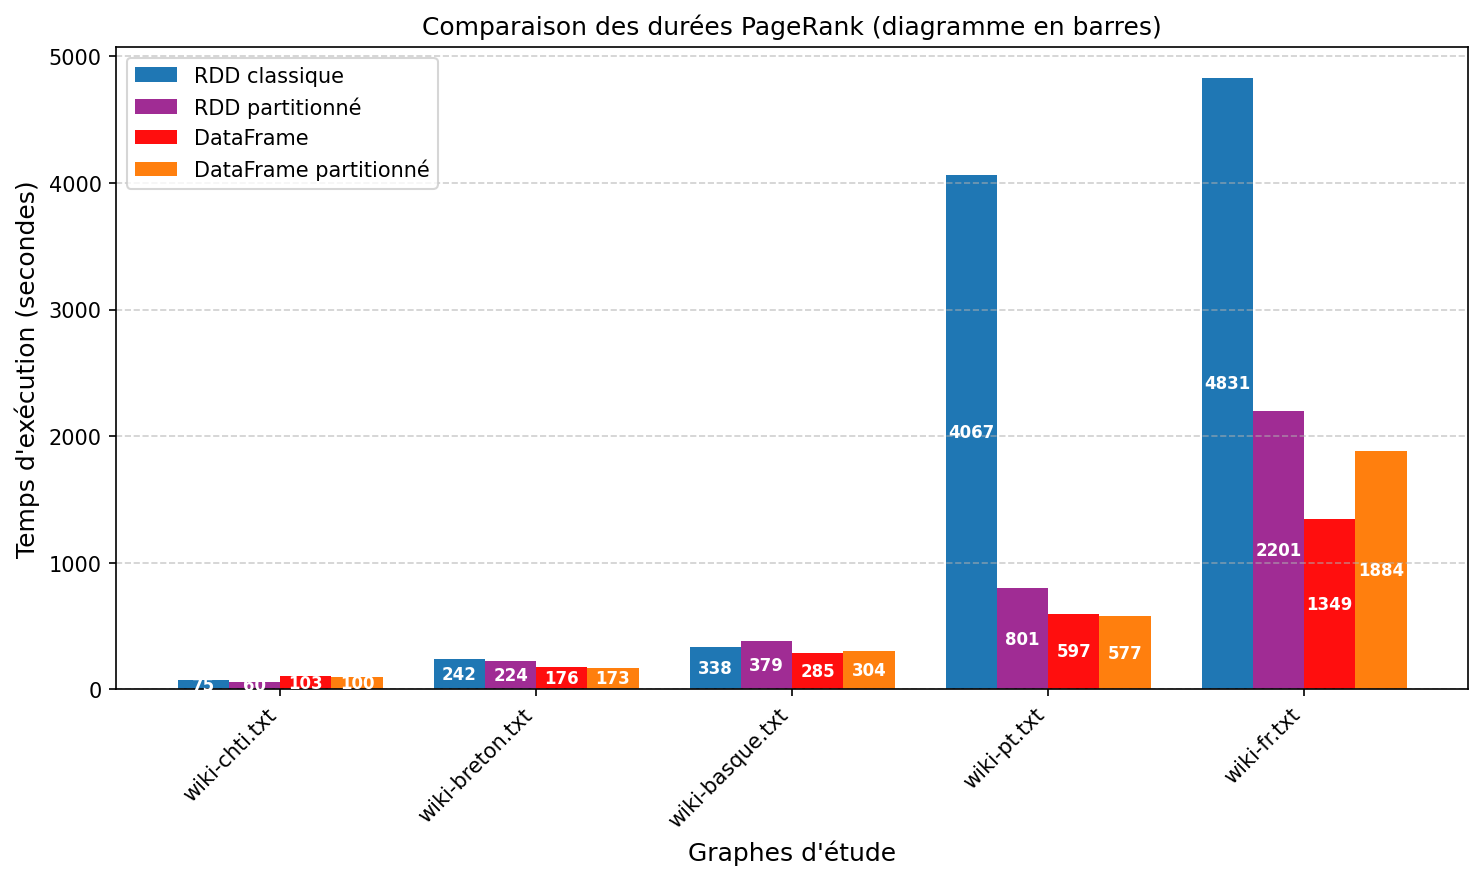
\includegraphics[width=0.45\textwidth]{figures/benchmark_times_bar}
    }

    \vspace{0.5em}
    \caption{Comparaison des temps d'exécution du \gls{pagerank} selon la taille des graphes et la structure de calcul utilisée.}
    \label{fig:benchmark_times}
\end{figure}

Les résultats présentés dans la \autoref{tab:benchmark_times} et illustrés par les figures~\ref{fig:benchmark_times_evolution} et~\ref{fig:benchmark_times_bar} permettent d'évaluer l'influence de la structure de calcul (\gls{rdd} ou \gls{dataframe}) et du partitionnement sur les performances globales de l'algorithme \gls{pagerank}.

\subsection{Comportement selon la taille des graphes}

Pour les graphes de petite à moyenne taille (\texttt{wiki-chti.txt}, \texttt{wiki-breton.txt} et \texttt{wiki-basque.txt}), les temps d'exécution observés restent comparables entre les quatre implémentations.  
Les différences mesurées demeurent faibles, avec un avantage marginal pour la structure \gls{rdd} classique.  
Cette tendance s'explique par la simplicité du modèle \gls{rdd}, dont la planification et la sérialisation impliquent une surcharge moindre que celle introduite par le moteur \gls{dataframe} et son optimiseur \gls{catalyst}.  
Dans ces conditions, la granularité fine du partitionnement ne procure pas de bénéfice significatif, le coût des opérations restant dominé par la lecture et la distribution initiale des données.

\subsection{Effet du partitionnement sur les grands graphes}

Lorsque la taille des graphes croît (\texttt{wiki-pt.txt} et \texttt{wiki-fr.txt}), les écarts de performance deviennent plus prononcés.  
L'implémentation \gls{rdd} partitionné réduit considérablement les temps d'exécution par rapport à la version non partitionnée, avec des gains pouvant atteindre 75~\%.  
Cette amélioration est directement liée à la réduction du nombre d'opérations de \textit{shuffle} et à une meilleure localité des données grâce à l'utilisation d'un \texttt{HashPartitioner} cohérent entre les transformations successives.  
Toutefois, malgré cette optimisation, le modèle \gls{rdd} partitionné demeure moins performant que les implémentations basées sur \gls{dataframe}, qui bénéficient d'un plan d'exécution optimisé et d'une gestion mémoire plus efficace.

\subsection{Limites du partitionnement manuel dans les DataFrames}

L'analyse met en évidence un comportement inattendu : la version \gls{dataframe} Partitionné présente des performances légèrement inférieures à la version \gls{dataframe} standard.  
Ce résultat suggère que le partitionnement manuel ne se substitue pas efficacement à la répartition automatique opérée par \gls{spark}.  
Les mécanismes internes d'optimisation, notamment le plan d'exécution adaptatif et la planification dynamique de \gls{catalyst}, permettent une répartition plus équilibrée des partitions entre les \textit{exécutors}.  
L'imposition d'un partitionnement fixe tend, au contraire, à restreindre la flexibilité du moteur et à accroître les échanges inter-partitions, ce qui explique la légère dégradation constatée.

\subsection{Synthèse des résultats}

L'étude des temps d'exécution permet de dégager plusieurs constats :
\begin{itemize}
    \item pour les graphes de petite et moyenne taille, les quatre approches présentent des performances similaires, avec une légère supériorité du modèle \gls{rdd} ;
    \item sur les graphes volumineux, le partitionnement améliore les performances du modèle \gls{rdd}, mais ce dernier reste inférieur à la version \gls{dataframe} en termes de rapidité ;
    \item le partitionnement manuel des \glspl{dataframe} ne procure pas de bénéfice et tend à perturber les optimisations automatiques du moteur \gls{spark}.
\end{itemize}

Ces observations mettent en évidence le rôle central de la stratégie de partitionnement dans les traitements distribués à grande échelle.  
Elles confirment également que les optimisations internes des \glspl{dataframe} surpassent, dans la majorité des cas, les réglages manuels effectués sur les structures \gls{rdd}, en particulier lorsque la volumétrie du graphe devient importante.

Abordons à présent une étude plus précise des temps d'exécution sur la base des quatre opérations : \texttt{map}, \texttt{flatMap}, \texttt{sum} et \texttt{count}.

\section{Analyse des temps d'exécution par opération}

Sur la base des résultats précédents, il semble pertinent d'étudier plus finement les temps d'exécution selon les quatre opérations décrites ci-après et qui reflètent directement les coûts associés aux transformations et aux actions appliquées aux données distribuées :

\begin{itemize}
    \item \textbf{\texttt{map}} : applique une fonction à chaque élément du \gls{rdd} ou du \gls{dataframe}.  
    Cette opération est purement locale et s'exécute indépendamment sur chaque partition.  
    L'analyse de son temps d'exécution permet d'évaluer l'efficacité du traitement élémentaire et la gestion interne de la parallélisation.

    \item \textbf{\texttt{flatMap}} : étend la transformation précédente en produisant plusieurs éléments de sortie pour chaque élément d'entrée.  
    Elle intervient notamment dans la construction du graphe et la propagation des contributions lors du calcul du \gls{pagerank}.  
    Son coût est plus sensible à la structure des données et au volume intermédiaire généré, ce qui en fait un bon indicateur de la surcharge de \textit{sérialisation} et des transferts réseau.

    \item \textbf{\texttt{sum}} : agrège l'ensemble des valeurs numériques distribuées au sein du \gls{cluster}.
    Cette opération déclenche un processus de réduction global impliquant des échanges inter-partitions.  
    L'analyse de ses performances renseigne sur l'efficacité des agrégations et sur la latence des communications entre \textit{executors}.

    \item \textbf{\texttt{count}} : évalue le nombre total d'éléments dans la structure de données.  
    A première vue simple, cette action force l'exécution complète du plan de calcul et permet ainsi de mesurer le coût global de matérialisation des transformations précédentes.  
    Elle constitue un indicateur pertinent de la charge d'exécution effective et du coût des opérations de lecture et de synchronisation.
\end{itemize}

L'étude de ces quatre opérations offre une vision complémentaire aux mesures globales du tableau \autoref{tab:benchmark_times}.  
Elle permet d'isoler les facteurs qui influencent le plus directement les performances, tels que la localité des calculs, la \textit{sérialisation} des objets, le volume de données échangé ou encore la stratégie d'évaluation paresseuse (\textit{lazy evaluation}) propre à \gls{spark}.

Les figures~\ref{fig:wiki-chti_ops_nogc} à~\ref{fig:wiki-fr_ops_gc} présentent la durée des principales opérations (\texttt{map}, \texttt{flatMap}, \texttt{sum}, \texttt{count}) pour chaque structure de calcul et chaque graphe, avec et sans prise en compte du temps consacré au \textit{garbage collector}.  
Les graphiques de gauche illustrent les temps d'exécution bruts, tandis que ceux de droite intègrent le surcoût lié à la gestion mémoire.

L'analyse met en évidence que l'implémentation \gls{dataframe} ne mobilisant pas les opérations \texttt{map} et \texttt{flatMap}, à la différence de l'approche en \gls{rdd}, constitue un premier facteur explicatif de la meilleure efficacité des \glspl{dataframe}, en limitant le nombre de transformations explicites sur les partitions.

Concernant les opérations \texttt{sum} et \texttt{count}, bien que les temps globaux soient supérieurs pour les petits graphes avec la structure \gls{dataframe} (voir \autoref{fig:benchmark_times}), ces opérations sont exécutées plus rapidement que dans les \glspl{rdd}.  
Ce comportement s'explique par la surcharge initiale du moteur \gls{catalyst}, responsable de la génération et de l'optimisation du plan d'exécution.  
Sur de petits volumes de données, cette phase d'analyse et de planification introduit un coût fixe significatif, masquant les gains offerts par les optimisations internes.  
Lorsque la taille du graphe croît, ce coût devient marginal et les optimisations de \gls{catalyst} se traduisent par une réduction sensible du temps total d'exécution.

Enfin, le temps induit par le \textit{garbage collector} croît proportionnellement à la taille des graphes et au volume de mémoire utilisé.  
Pour les graphes les plus volumineux, tels que \texttt{wiki-pt.txt} et \texttt{wiki-fr.txt}, ce coût devient particulièrement marqué dans l'implémentation \gls{rdd} sans partitionnement, où la gestion mémoire génère une surcharge importante.  
Cette contrainte explique la baisse notable de performance observée pour les graphes denses, en raison de l'augmentation de la fréquence et de la durée des cycles de nettoyage.

\clearpage

\begin{figure*}[ht]
    \centering
    \resizebox{0.92\textwidth}{!}{%
        \begin{minipage}{\textwidth}

    % === Ligne 1 : wiki-chti ===
    \subfloat[\textbf{wiki-chti — sans GC}\label{fig:wiki-chti_ops_nogc}]{
        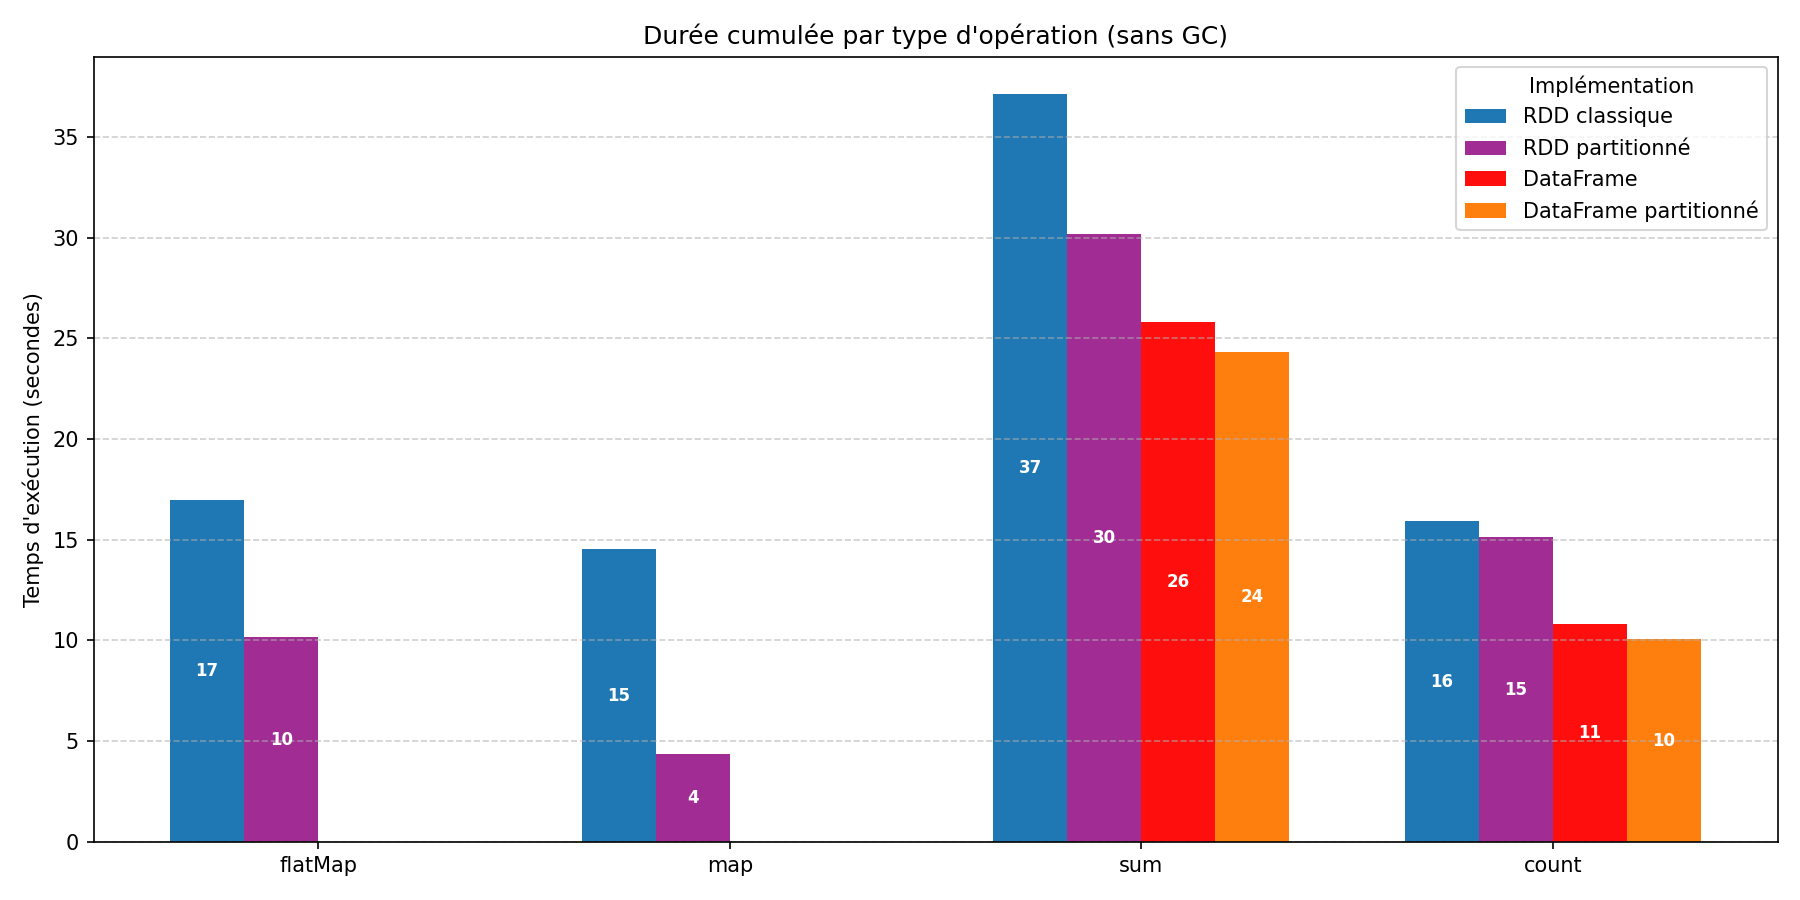
\includegraphics[width=0.45\textwidth]{figures/wiki-chti_ops_duration_core_nogc_labels}
    }\hfill
    \subfloat[\textbf{wiki-chti — avec GC}\label{fig:wiki-chti_ops_gc}]{
        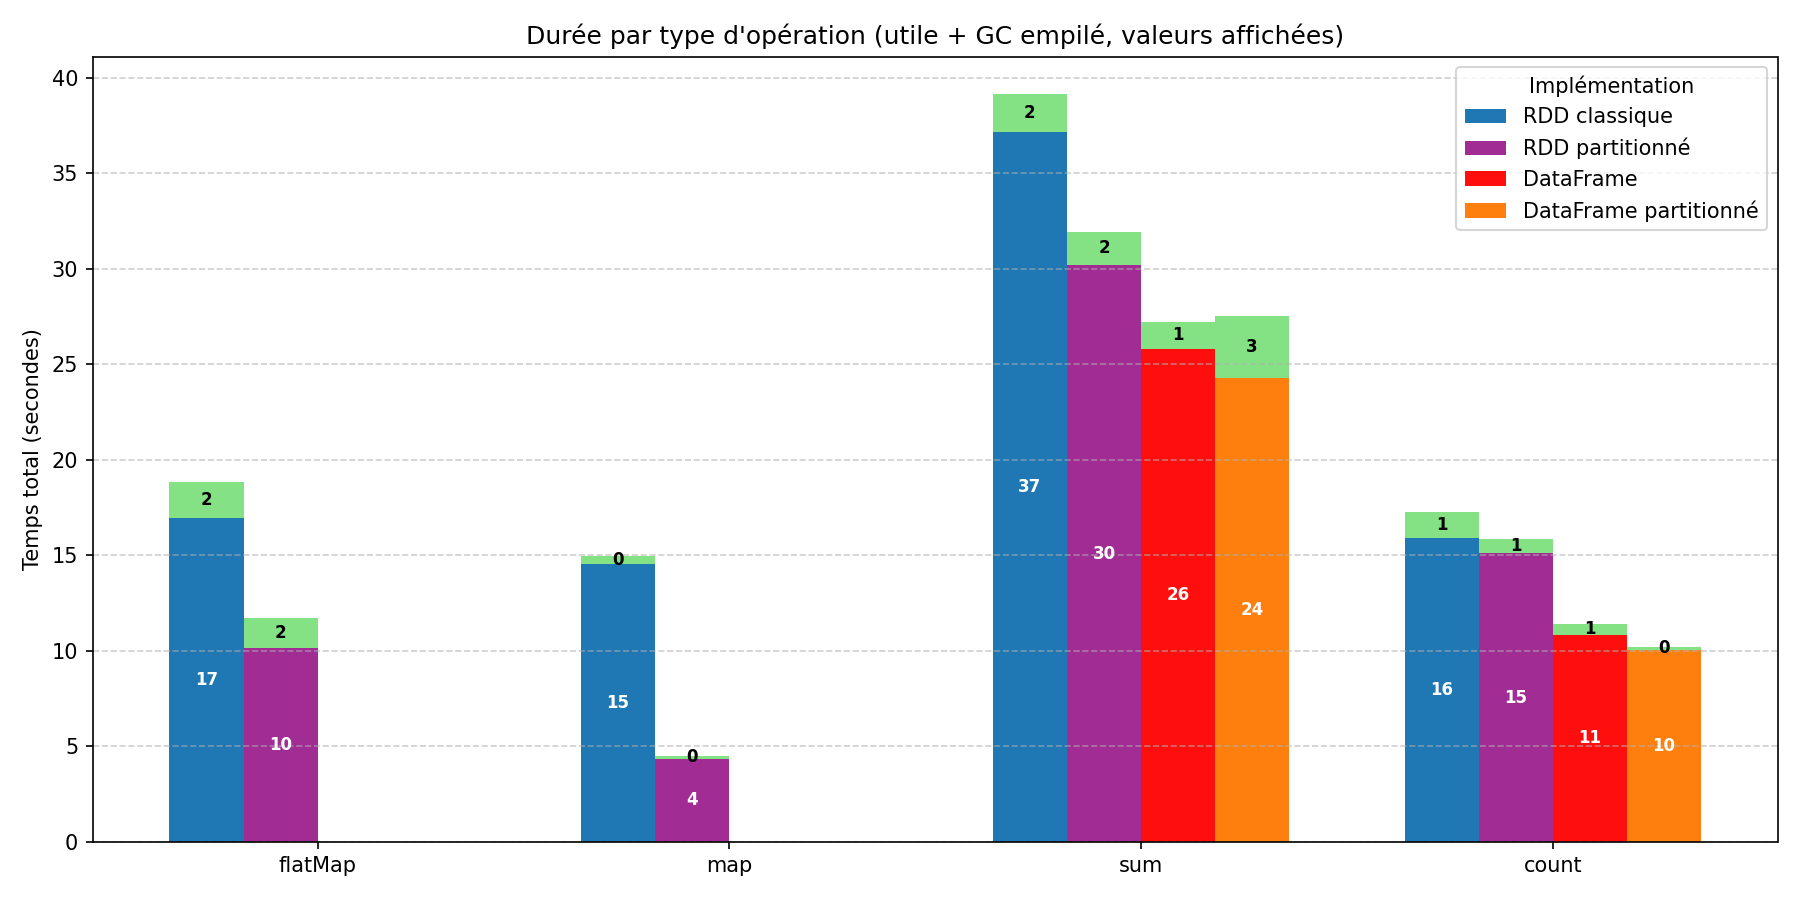
\includegraphics[width=0.45\textwidth]{figures/wiki-chti_ops_duration_core_with_gc_labels}
    }

    \vspace{0.2em}

    % === Ligne 2 : wiki-breton ===
    \subfloat[\textbf{wiki-breton — sans GC}\label{fig:wiki-breton_ops_nogc}]{
        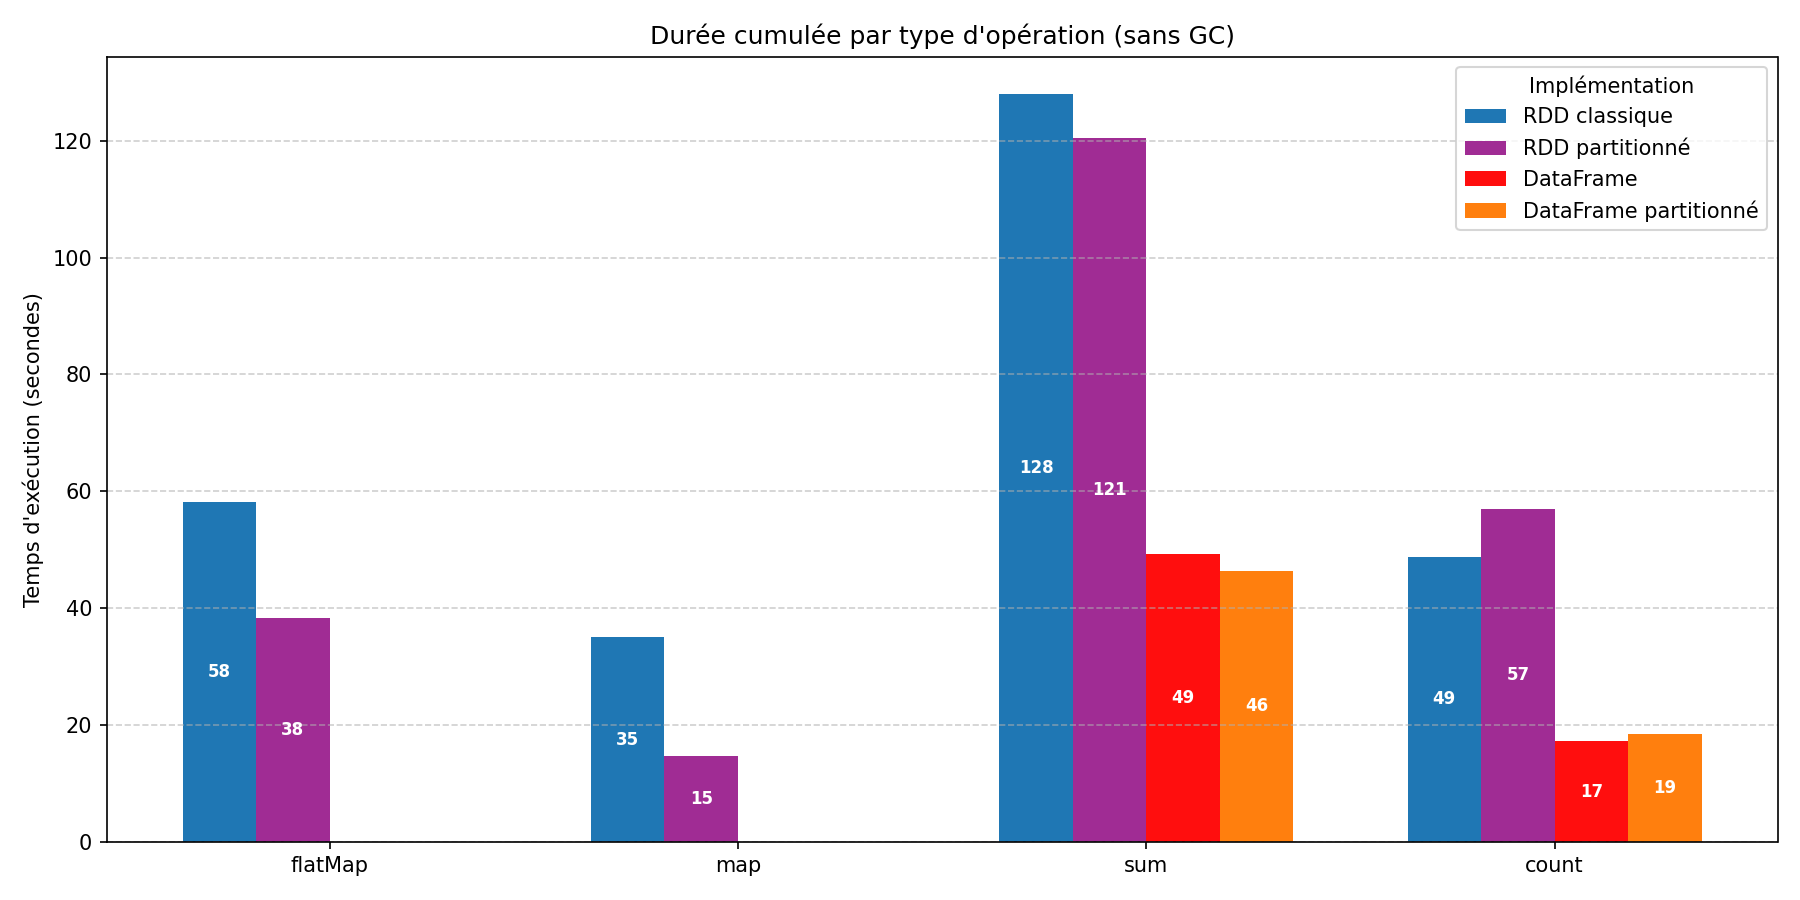
\includegraphics[width=0.45\textwidth]{figures/wiki-breton_ops_duration_core_nogc_labels}
    }\hfill
    \subfloat[\textbf{wiki-breton — avec GC}\label{fig:wiki-breton_ops_gc}]{
        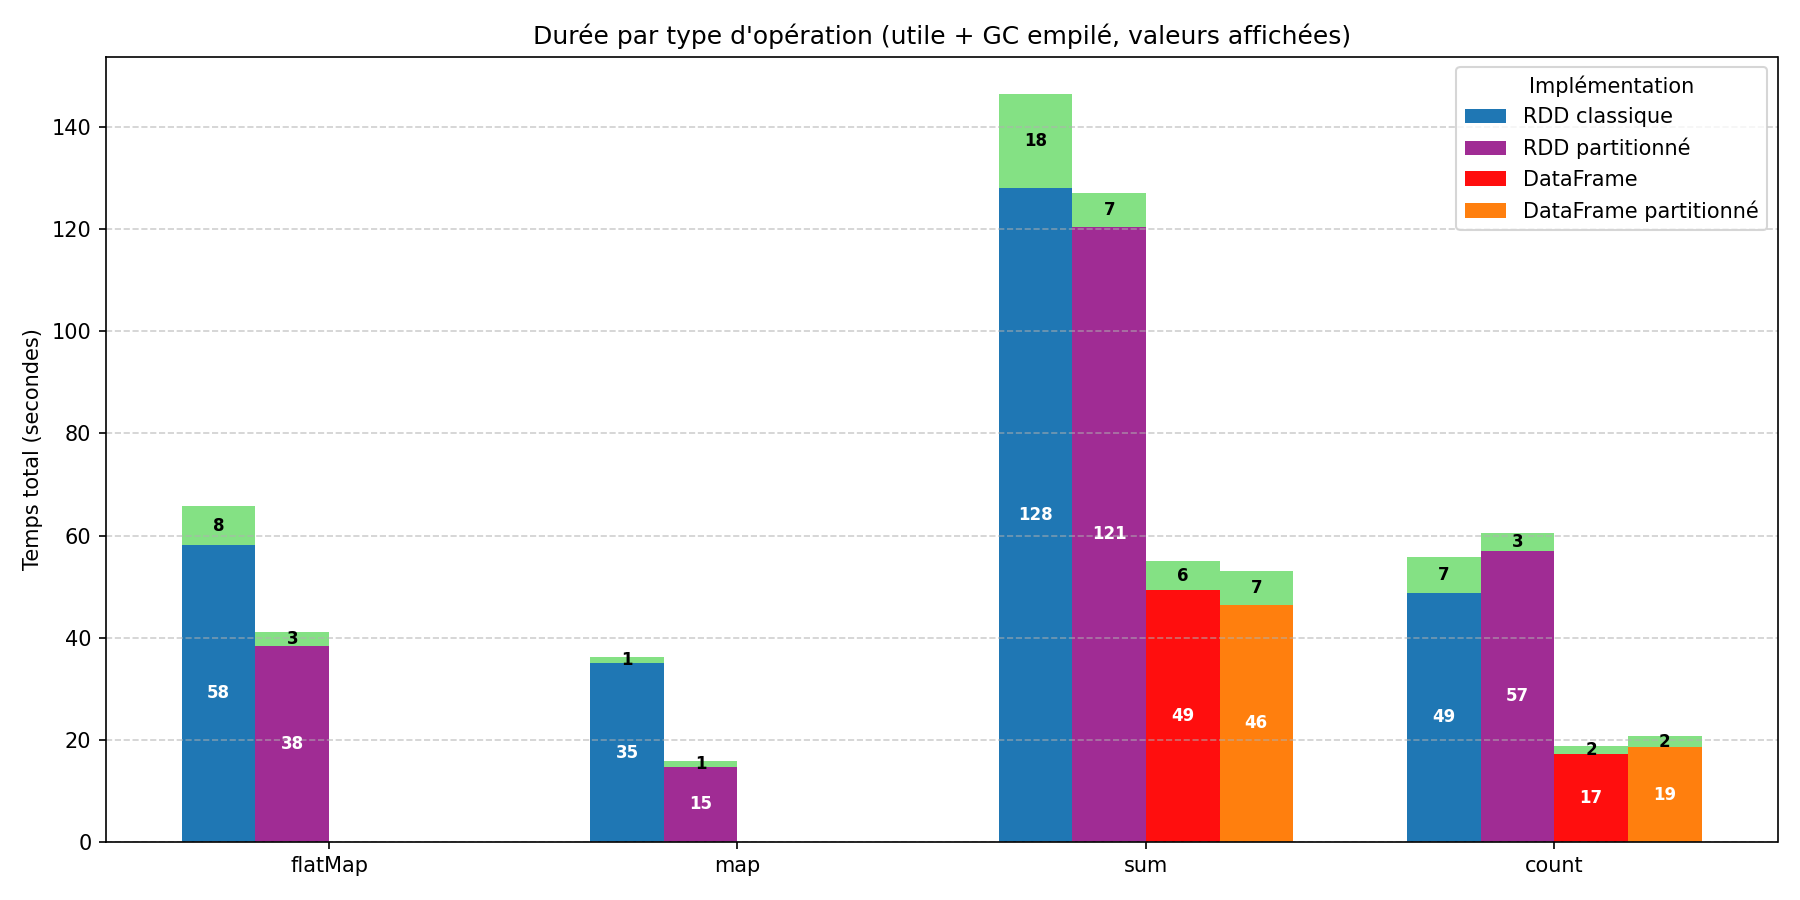
\includegraphics[width=0.45\textwidth]{figures/wiki-breton_ops_duration_core_with_gc_labels}
    }

    \vspace{0.2em}

    % === Ligne 3 : wiki-basque ===
    \subfloat[\textbf{wiki-basque — sans GC}\label{fig:wiki-basque_ops_nogc}]{
        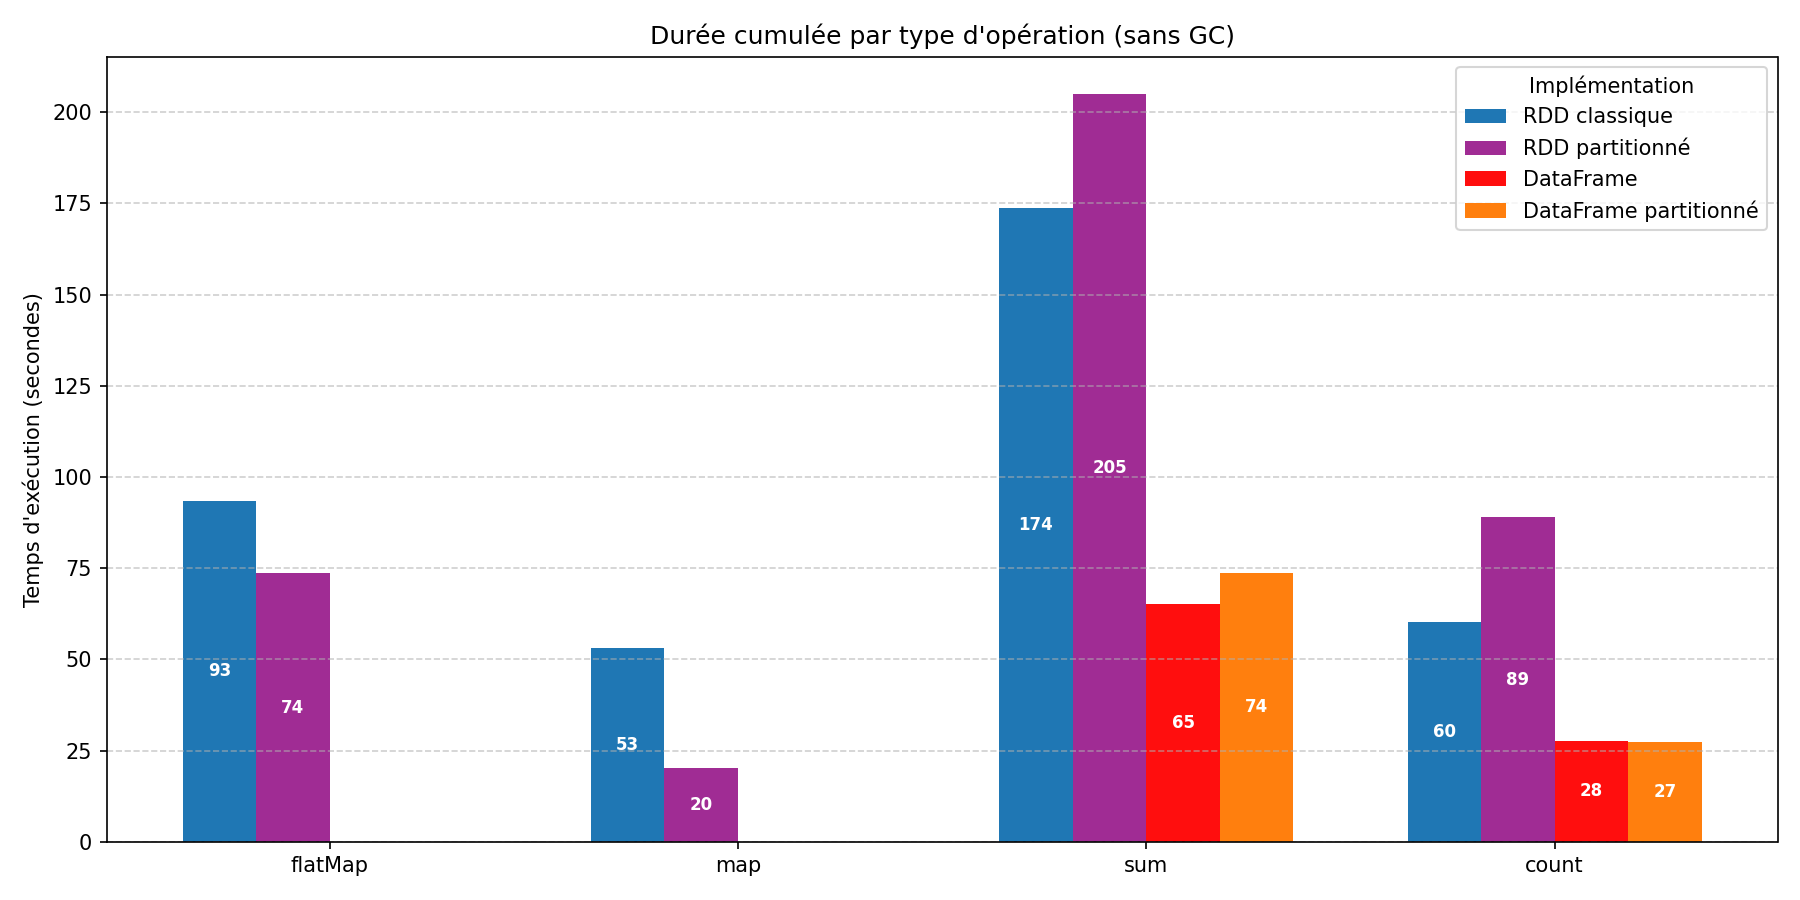
\includegraphics[width=0.45\textwidth]{figures/wiki-basque_ops_duration_core_nogc_labels}
    }\hfill
    \subfloat[\textbf{wiki-basque — avec GC}\label{fig:wiki-basque_ops_gc}]{
        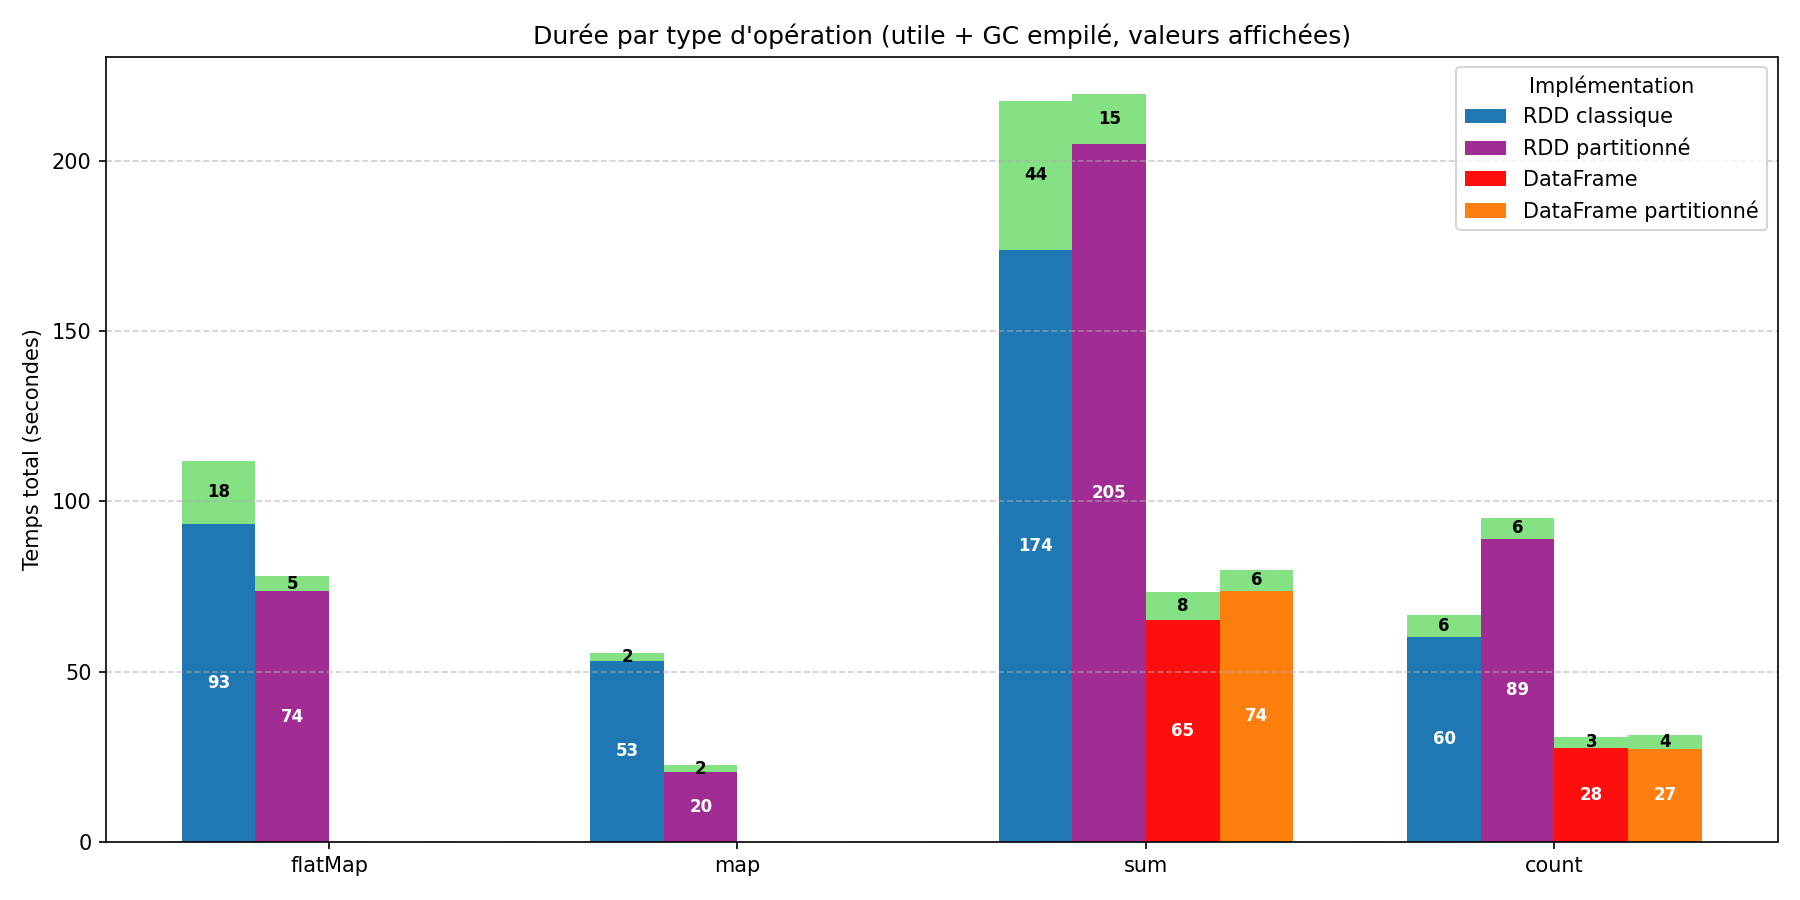
\includegraphics[width=0.45\textwidth]{figures/wiki-basque_ops_duration_core_with_gc_labels}
    }

    \vspace{0.2em}

    % === Ligne 4 : wiki-pt ===
    \subfloat[\textbf{wiki-pt — sans GC}\label{fig:wiki-pt_ops_nogc}]{
        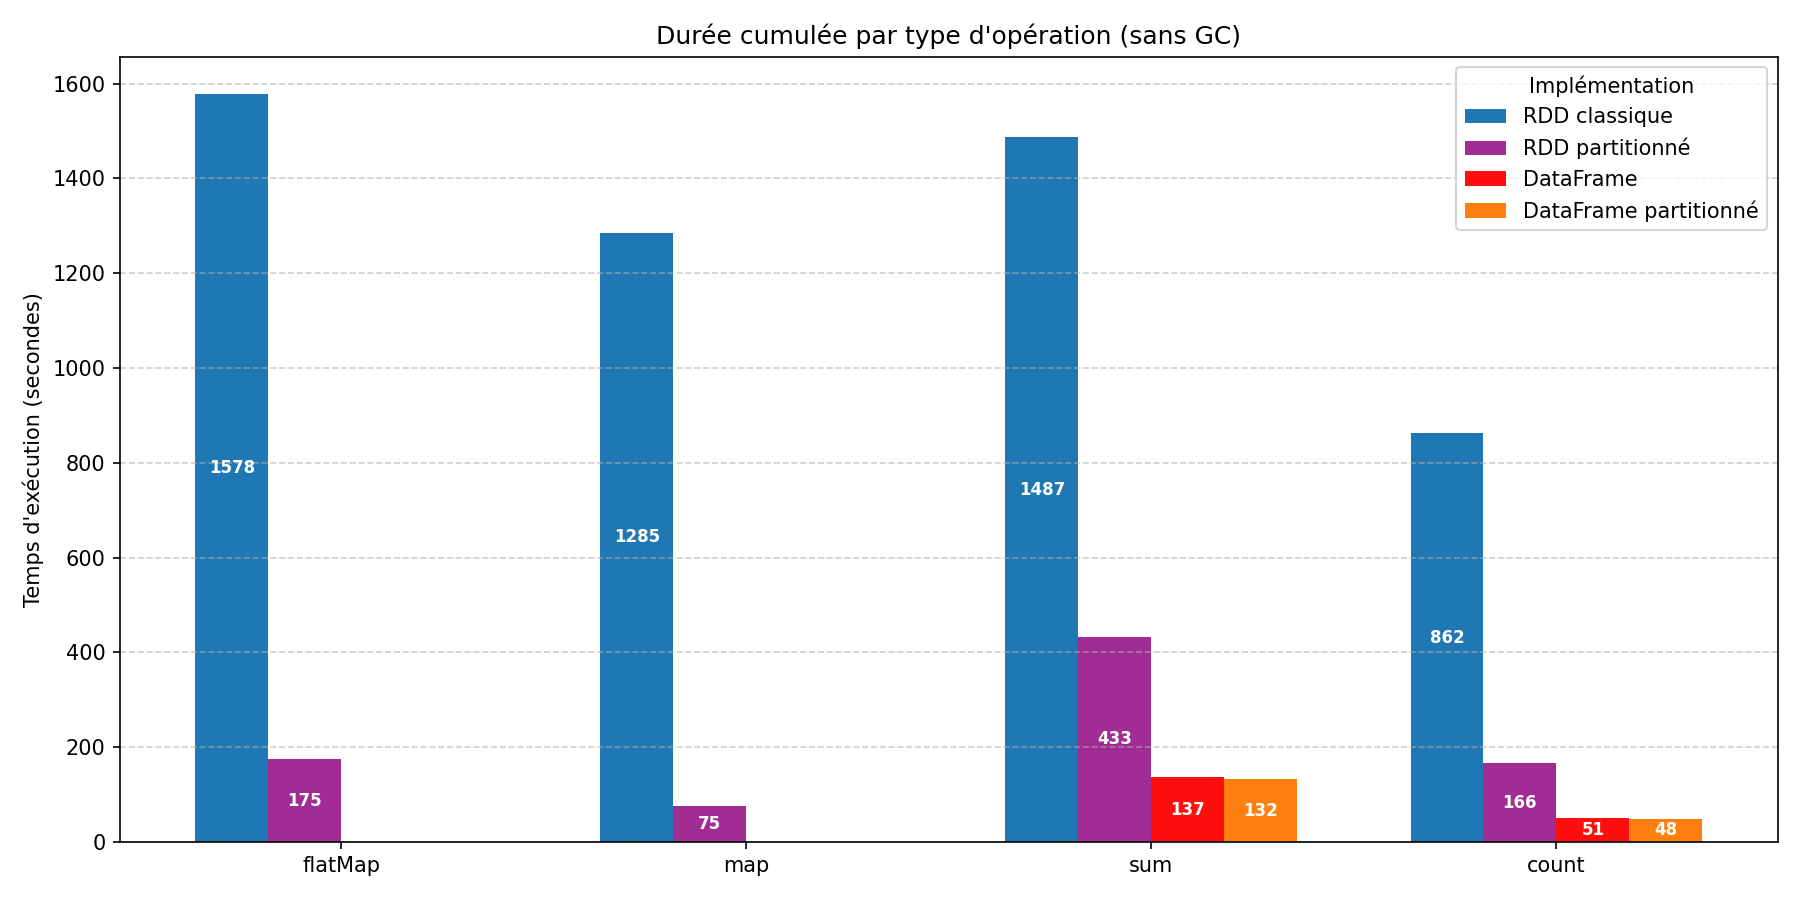
\includegraphics[width=0.45\textwidth]{figures/wiki-pt_ops_duration_core_nogc_labels}
    }\hfill
    \subfloat[\textbf{wiki-pt — avec GC}\label{fig:wiki-pt_ops_gc}]{
        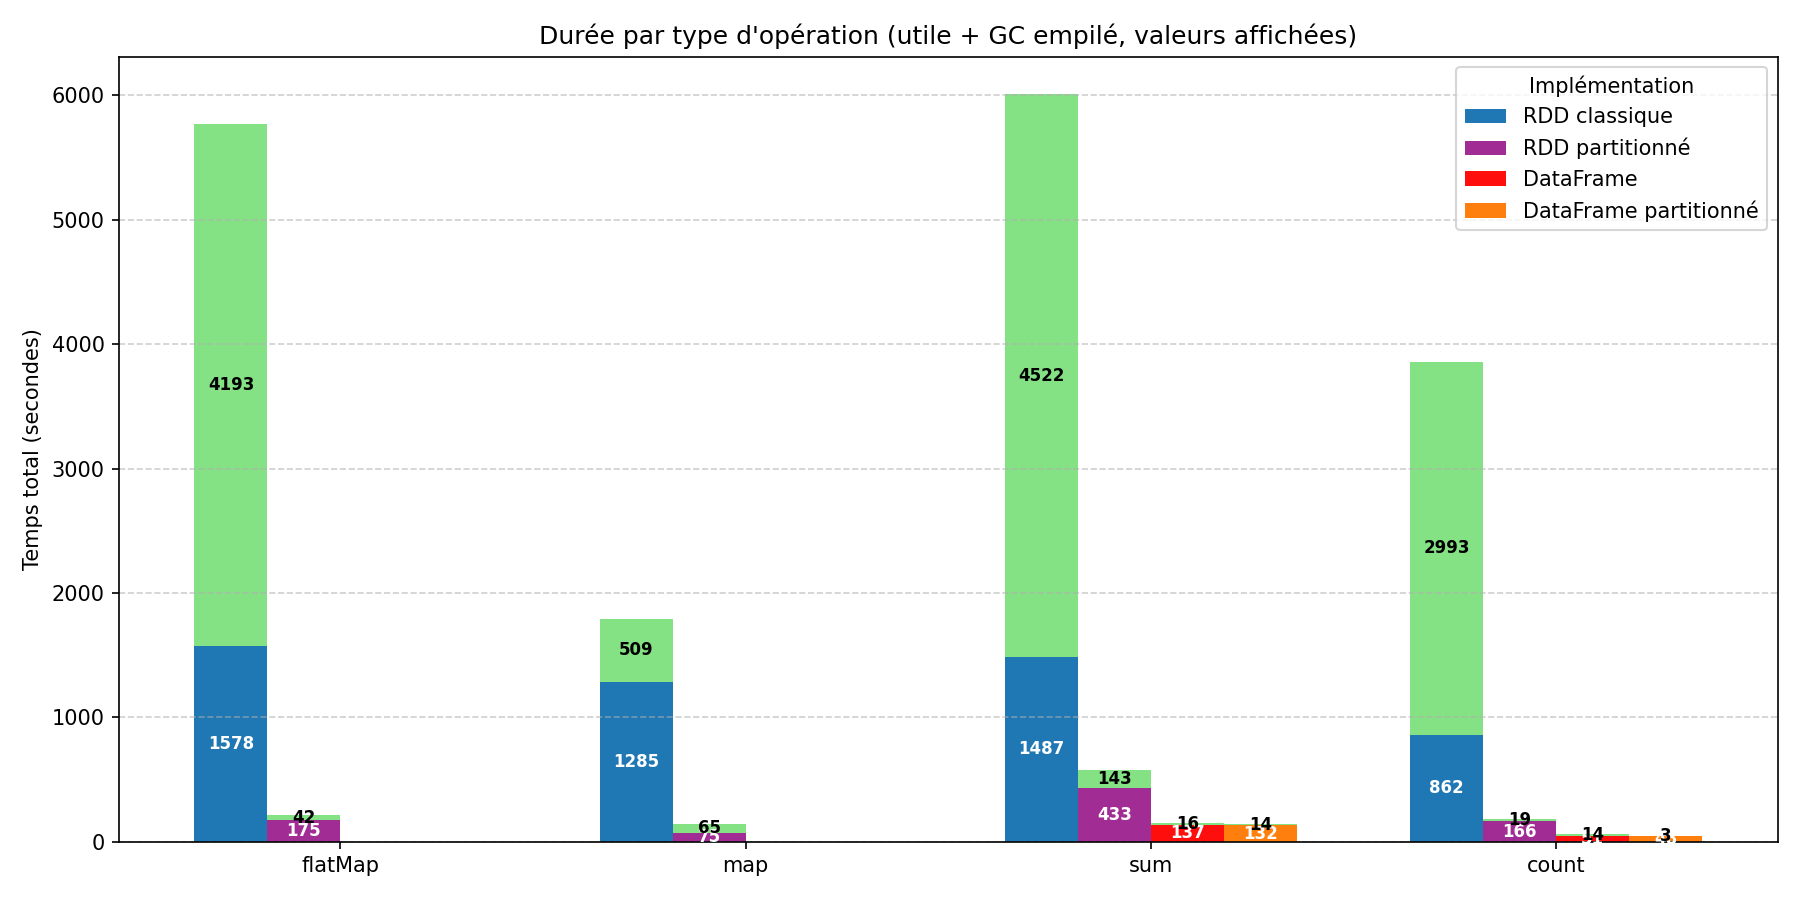
\includegraphics[width=0.45\textwidth]{figures/wiki-pt_ops_duration_core_with_gc_labels}
    }

    \vspace{0.2em}

    % === Ligne 5 : wiki-fr ===
    \subfloat[\textbf{wiki-fr — sans GC}\label{fig:wiki-fr_ops_nogc}]{
        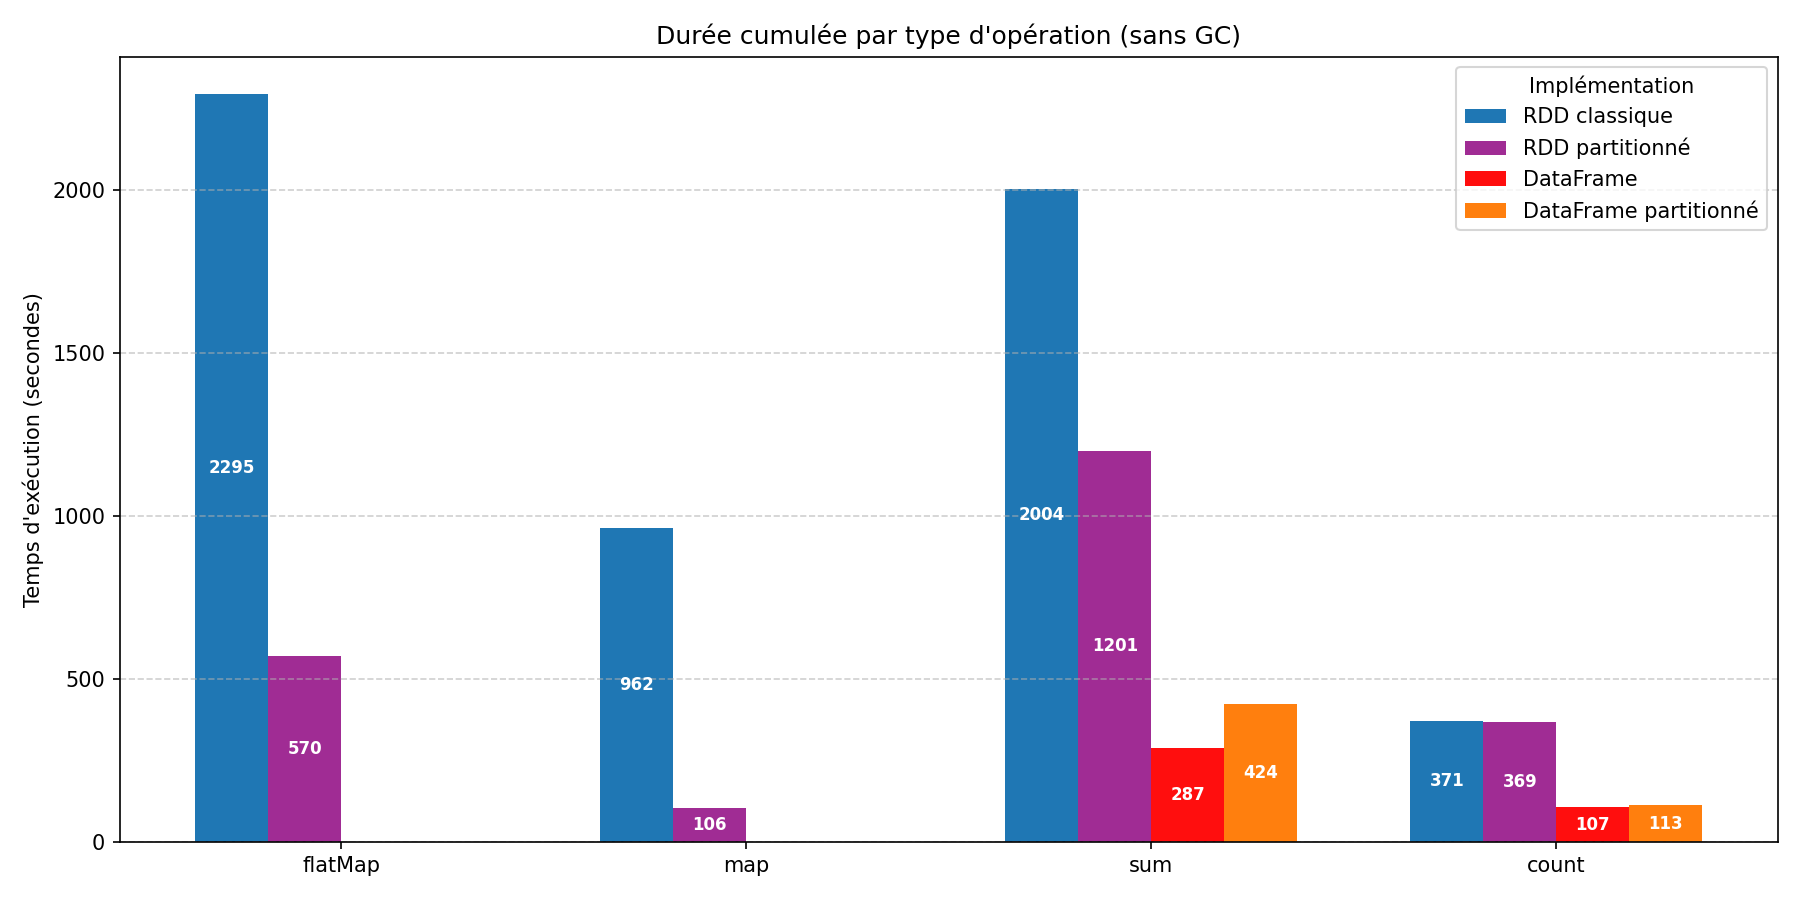
\includegraphics[width=0.45\textwidth]{figures/wiki-fr_ops_duration_core_nogc_labels}
    }\hfill
    \subfloat[\textbf{wiki-fr — avec GC}\label{fig:wiki-fr_ops_gc}]{
        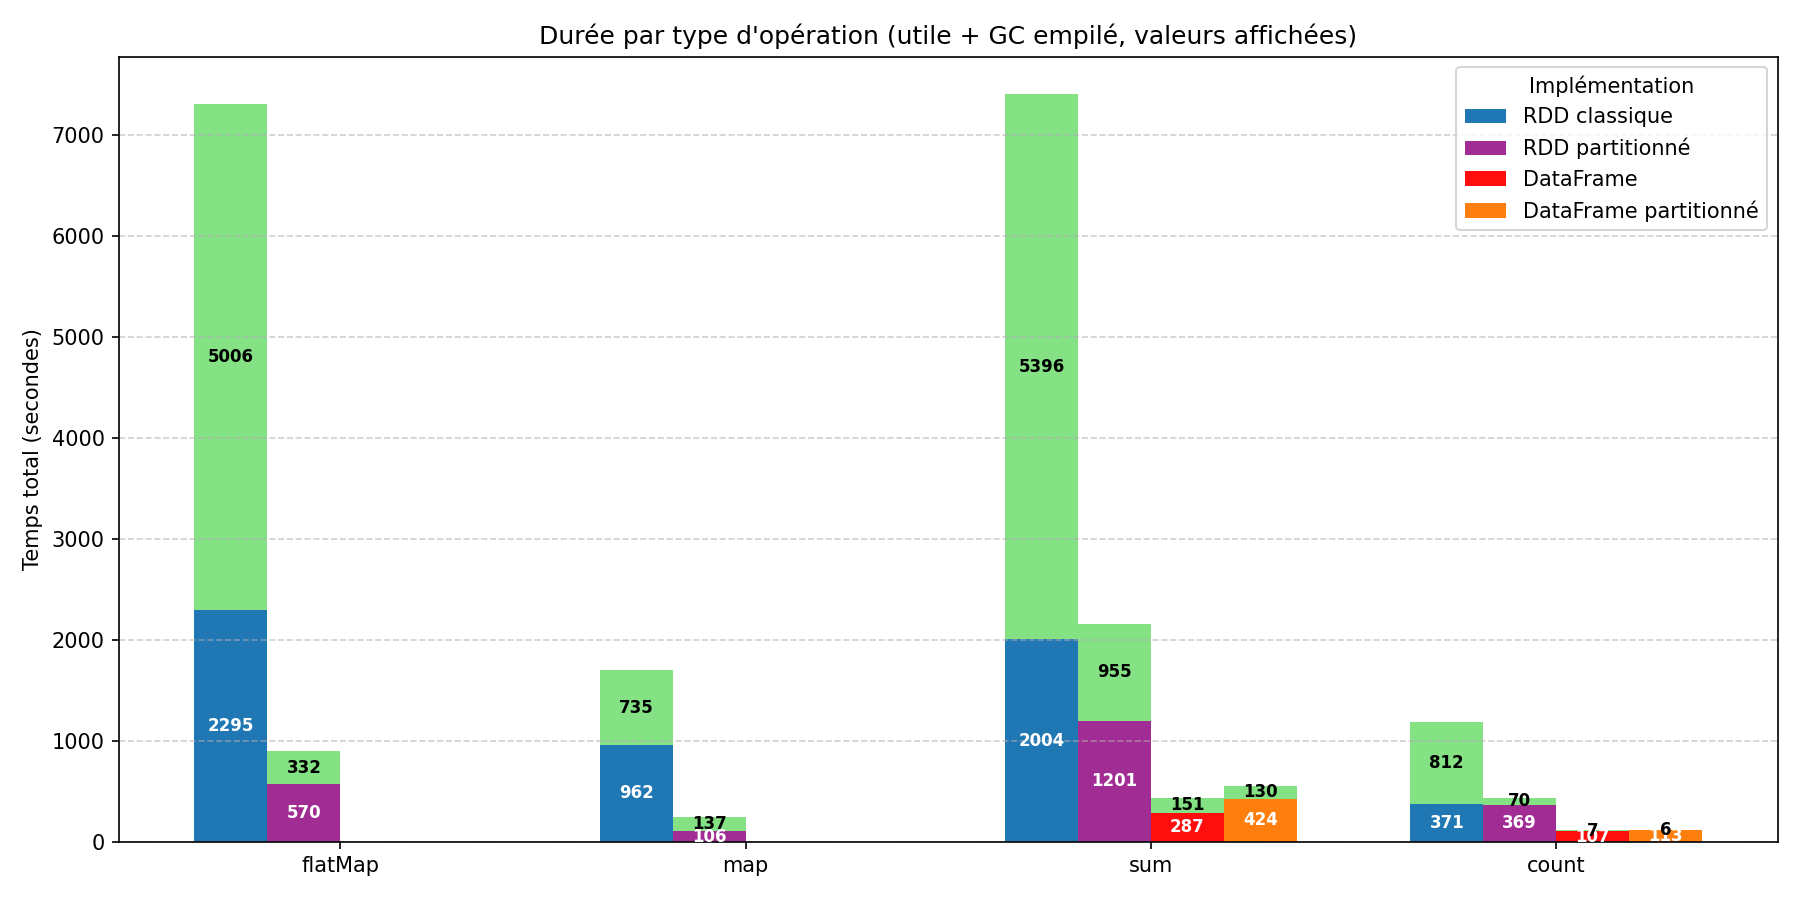
\includegraphics[width=0.45\textwidth]{figures/wiki-fr_ops_duration_core_with_gc_labels}
    }

        \end{minipage}%
    }

    \caption{Durée moyenne par type d'opération (\texttt{map}, \texttt{flatMap}, \texttt{sum}, \texttt{count}) 
    pour chaque structure de calcul et chaque graphe, avec et sans prise en compte du temps passé dans le \textit{garbage collector}.}
    \label{fig:ops_duration_gc_comparison}
\end{figure*}

\clearpage

\section{Conclusion}

L'étude présentée a permis d'analyser en profondeur l'implémentation de l'algorithme \gls{pagerank} sur la plateforme \gls{spark}, en comparant quatre structures de calcul : \gls{rdd}, \gls{rdd} partitionné, \gls{dataframe} et \gls{dataframe} partitionné.  
L'ensemble des expérimentations a été mené sur cinq graphes de tailles croissantes, à l'aide d'une configuration \gls{spark} optimisée, afin d'évaluer l'impact des choix d'implémentation sur les temps d'exécution et l'efficacité mémoire.

Les résultats ont mis en évidence plusieurs constats majeurs.  
Tout d'abord, pour les graphes de petite et moyenne taille, les structures \gls{rdd} offrent des performances comparables, voire légèrement supérieures, à celles des \glspl{dataframe}.  
Cependant, à mesure que la taille du graphe augmente, les \glspl{dataframe} tirent parti du moteur d'optimisation \gls{catalyst}, qui améliore la planification et la réduction des échanges réseau, leur conférant une meilleure scalabilité.

L'introduction d'un partitionnement explicite s'est révélée bénéfique pour les \glspl{rdd}, réduisant de manière significative les coûts liés aux \textit{shuffles} et à la communication inter-nœuds.  
Cette optimisation permet d'obtenir un gain de performance notable sur les graphes volumineux, bien que l'implémentation reste moins efficace que celle basée sur les \glspl{dataframe}.  
À l'inverse, le partitionnement manuel des \glspl{dataframe} n'a pas apporté d'amélioration et a même diminuer les performances, confirmant que le moteur \gls{spark} gère déjà efficacement la distribution et l'adaptation du plan d'exécution à la taille du jeu de données.

L'analyse des durées d'exécution par type d'opération (\texttt{map}, \texttt{flatMap}, \texttt{sum}, \texttt{count}) a montré que les \glspl{dataframe} réduisent significativement le coût de ces opérations grâce à une exécution vectorisée et une meilleure gestion mémoire.  
De plus, l'étude du \textit{garbage collector} a souligné son impact croissant sur les performances, notamment pour les graphes de grande taille, où il devient un facteur limitant dans le cas des \glspl{rdd} non partitionnés.

En conclusion, il ressort de cette analyse que :
\begin{itemize}
    \item le partitionnement constitue une amélioration essentielle pour les \glspl{rdd}, leur permettant d'approcher les performances des \glspl{dataframe} ;
    \item les \glspl{dataframe} conservent un avantage global en termes de scalabilité et d'optimisation automatique ;
    \item la surcharge induite par le moteur \gls{catalyst} devient négligeable pour les graphes de grande taille, mais pénalise les petits jeux de données ;
    \item la gestion de la mémoire et du \textit{garbage collector} représente un axe critique d'optimisation pour les traitements distribués de grande échelle.
\end{itemize}

Ces observations ouvrent la voie à des perspectives d'amélioration, notamment par l'intégration de mécanismes de partitionnement adaptatif, l'étude de formats de stockage optimisés (par exemple \gls{parquet}) ou encore l'analyse de l'impact du paramétrage du \textit{garbage collector} sur les performances globales.  
De telles optimisations permettraient d'affiner la gestion des ressources et d'améliorer la stabilité temporelle des traitements à grande échelle.

\clearpage

\printglossary[type=\acronymtype, title={Liste des acronymes}]
\printglossary[title={Glossaire}]

\printbibliography[title={Bibliographie}]

\end{document}
